%%
%% TeX:UTF-8
%%
%% POSTECH 학위논문양식 LaTeX용 (ver 0.4) 예시
%%
%% @version 0.6
%% @author  박준신 Junshin Park (mailto:lonelywing@postech.ac.kr)
%% @date    2021. 3. 24.
%%
%% @requirement
%% teTeX, fpTeX, teTeX 등의 LaTeX2e 배포판
%% + 은광희 님의 HLaTeX 0.991 이상 버젼 또는 홍석호 님의 HPACK 1.0
%% : 설치에 대한 자세한 정보는 http://www.ktug.or.kr을 참조바랍니다.
%%
%% @Tested in
%% Windows 7, Texlive 2014.
%% Ubuntu 14.04 LTS, Texlive 2016.
%% Compatibility with miktex has not been tested yet.
%%
%% @note for international students
%% Present format is intended for both Korean and international students.
%% For those control statements or arguments that need guidance,
%% comments are added in both languages for convenience. You may however delete the Korean comments
%% if your specific environment does not support Korean.
%% For more information or help, please contact the author of which email address is written above.
%%
%%
%% @acknowledgement
%% 본 latex template은 kaist 채승병님의 template을 바탕으로 만들어졌음을 밝힙니다.
%% Alpha test 및 본 thesis 예시 내용은 컴퓨터공학과 졸업생이신 오수영 학우의 도움으로 작성되었습니다.
%% 또한, Sae Hee Ryu의 지원이 한 스푼 들어갔습니다.
%% -------------------------------------------------------------------
%% @information
%% 이 예제 파일은 hangul-ucs를 사용합니다. UTF-8 입력 인코딩으로
%% 작성되었습니다. hlatex의 hfont는 이용하지 않습니다. --2006/02/11



% @class postech-ucs.cls
% @options [default: doctor, korean, final]
% - doctor: 박사과정 | master : 석사과정
% - korean: 한글논문 | english: 영문논문
% - final : 최종판   | draft  : 시험판
% - pdfdoc : 선택하지 않으면 북마크와 colorlink를 만들지 않습니다.(Generate bookmark and colorlink if enabled)
\documentclass[master,english,final]{postech-ucs}
%\documentclass[master,english,final]{postech-ucs}
% If you want make pdf document (include bookmark, colorlink)
%\documentclass[doctor,english,final,pdfdoc]{postech-ucs}

% postech-ucs.cls 에서는 기본으로 dhucs, ifpdf, graphicx, afterpage, refcount 패키지가 로드됩니다.
% (postech-ucs.cls by default loads dhucs, ifpdf,refcount and graphicx packages. Please load any additional packages if needed)
% 추가로 필요한 패키지가 있다면 주석을 풀고 적어넣으십시오,
%\usepackage{...}
\usepackage{amsmath}
\usepackage{enumitem}
\usepackage{algorithm}
\usepackage{algpseudocode}
\usepackage{comment}
\usepackage{physics}
\usepackage{anyfontsize}
\usepackage{lipsum}
\usepackage{amsfonts}
\usepackage{wrapfig}
\usepackage{subfigure}
\usepackage{graphicx}
\usepackage{caption}
\usepackage{multirow}
\usepackage{tabularx}
\usepackage{makecell}
\usepackage{placeins}
\usepackage{subcaption}

% \usepackage{bbm}
% \renewcommand{\thealgorithm}{}
\newcommand{\argmax}{\operatornamewithlimits{arg\,max}}

% @command title 논문 제목(title of thesis)
% @options [default: (none)]
% - korean: 한글제목(korean title) | english: 영문제목(english title)
\title[korean]{신경 상미분방정식을 사용한 분리된 표시 시간점 프로세스}
\title[english]{Decoupled Marked Temporal Point Process using Neural ODEs}

% @note 표지에 출력되는 제목을 강제로 줄바꿈하려면 \linebreak 을 삽입.
%       \\ 나 \newline 등을 사용하면 안됩니다. (아래는 예시)
%
% If you want to begin a new line in cover, use \linebreak .
% See examples above.
%


% @command author 저자 이름
% @param   family_name, given_name 성, 이름을 구분해서 입력
% @options [default: (none)]
% - korean: 한글이름 | chinese: 한문이름 | english: 영문이름
% ex) \author[english]{family name in english}{given name in english}
%
% If you are a foreigner (this means you have no korean name),
% You must fill the korean name as blank, instead of deleting it or commenting it out.
% \author[korean]{}{}
% \author[english]{Donald}{Trump}
%
%
\author[korean]{송}{유지}
\author[english]{Song}{Yujee}

% @command advisor 지도교수 이름 (복수가능)
% @usage   \advisor[options]{...한글이름...}{...영문이름...}{signed|nosign}
% @options [default: major]
% - major: 주 지도교수  | coopr: 공동 지도교수
\advisor[major]{김 원 화}{Won Hwa Kim}{nosign}
%
% 지도교수 한글이름은 입력하지 않아도 됩니다.
% You may not input advisor's korean name
% like this \advisor[major]{}{Chang, Kee Joo}{signed}
%

% @command department {학과이름}{학위종류} - 아래 표에 따라 코드를 입력
% @command department {department code}{degree field}
%
% department code table
% https://postech.ac.kr/admission-education/graduate/ 정보 및 순서를 따름
% MA    // 수학             Department of Mathematics
% PH    // 물리             Department of Physics
% CH    // 화학             Department of Chemistry
% LS    // 생명             Department of Life Sciences
% MS    // 신소재           Department of Materials Science and Engineering
% ME    // 기계             Department of Mechanical Engineering
% IME   // 산경             Department of Industrial and Management Engineering
% EE    // 전자             Department of Electrical Engineering
% CSE   // 컴공             Department of Computer Science and Engineering
% CE    // 화공             Department of Chemical Engineering
% CITE  // 창의IT           Department of Creative IT Engineering
% EV    // 환경공학         Division of Environmental Science and Engineering
% GSAI  // 인공지능         Graduate School of Artificial Intelligence
% ITCE  // 정보전자융합공학 Division of IT Convergence Engineering
% AMS   // 첨단재료과학     Division of Advanced Material Science
% IBB   // 융합생명공학     Division of Integrative Biosciences and Biotechnology
% DANE  // 첨단원자력공학   Division of Advanced Nuclear Engineering
% I-BIO // 시스템생명공학   School of Interdisciplinary Bioscience and Bioengineering
% TIM   // 기술경영과정     Graduate Program for Technology and Innovation Management
% GIFT  // 철강에너지소재   Graduate Institute of Ferrous and Energy materials Technology

%
% science: 이학 | engineering: 공학 | business : 경영학
% 박사논문의 경우는 학위종류를 입력하지 않아도 됩니다.
% If you write Ph.D. dissertation, you cannot input degree field.

\department{GSAI}{}

% @command studentid 학번(ID)
\studentid{20232277}

% @command referee 심사위원 (석사과정 3인, 박사과정 5인)
\referee[1]{Won Hwa Kim}
\referee[2]{Dongwoo Kim}
\referee[3]{Sungsoo Ahn}
% Of course english name is available

% @command approvaldate 지도교수논문승인일
% @param   year,month,day 연,월,일 순으로 입력
\approvaldate{2024}{11}{27}

% @command refereedate 심사위원논문심사일
% @param   year,month,day 연,월,일 순으로 입력
\refereedate{2024}{11}{27}

% @command gradyear 졸업년도
\gradyear{2025}

% 본문 시작
\begin{document}

    % 앞표지, 속표지, 학위논문 제출승인서, 학위논문 심사완료 검인서는
    % 클래스 옵션을 final로 지정해주면 자동으로 생성되며,
    % 반대로 옵션을 draft로 지정해주면 생성되지 않습니다.

    % 영문초록 (abstract)
    \begin{abstract}
        A Marked Temporal Point Process (MTPP) is a stochastic process whose realization is a set of event-time data. 
MTPP is often used to understand complex dynamics of asynchronous temporal events such as money transaction, social media, healthcare, etc. 
Recent studies have utilized deep neural networks to capture complex temporal dependencies of events and generate embeddings that aptly represent the observed events. 
While most previous studies focus on the inter-event dependencies and their representations,
how individual events influence the overall dynamics over time has been under-explored. 
In this regime, we propose a Decoupled MTPP framework that disentangles characterization of a stochastic process into a set of evolving influences from different events. 
Our approach employs Neural Ordinary Differential Equations (Neural ODEs) \cite{bib:node} to learn flexible continuous dynamics of these influences while simultaneously addressing multiple inference problems, 
such as density estimation and survival rate computation. 
We emphasize the significance of disentangling the influences by comparing our framework with state-of-the-art methods on real-life datasets, 
and provide analysis on the model behavior for potential applications.
    \end{abstract}

    % 목차 (Table of Contents) 생성
    \tableofcontents

    % 표목차 (List of Tables) 생성
    \listoftables

    % 그림목차 (List of Figures) 생성
    \listoffigures

    % 위의 세 종류의 목차는 한꺼번에 다음 명령으로 생성할 수도 있습니다.
    %\makecontents

%% 이하의 본문은 LaTeX 표준 클래스 report 양식에 준하여 작성하시면 됩니다.
%% 하지만 part는 사용하지 못하도록 제거하였으므로, chapter가 문서 내의
%% 최상위 분류 단위가 됩니다.
%% You cannot use 'part'

\chapter{Introduction}
% Event-time data, which are found across various practical domains such as social media \cite{seismic, snapnets}, healthcare \cite{bib:RMTPP, meng2023dynamic} and stock changes \cite{Bacry2014MarketIA, hawkesInFinance}, 
comprise timelines of events of diverse types. 
Modeling such temporal data as a stochastic process, one seeks to predict time and type of the future events based on the history, i.e., previously observed sequential events. 
For example, a history of purchases of a person may tell when the person will buy a new item, and a short message from a famous social media influencer could affect a critical bull or bear in a stock market. %predicting an interaction in social media, purchase of an item in an online store, occurrence of disease based on history of diagnosis, etc.
Predicting such a future event is often realized as a chance of the event, i.e., a likelihood of the event $e$ at a specific time $t$, 
which constitutes a probability distribution function (pdf) $f(e,t)$. 

Classically, the event prediction has been handled using a Temporal Point Process (TPP), which is a stochastic process whose realization is a set of ordered time \cite{lec:tpp}. %Considering it as a random process, 
TPP characterizes at which time point an event will occur given historical time points. 
Hawkes Process effectively models this stochastic behavior by defining an \textit{conditional intensity function} which leverages the sum of excitation functions induced by past events called ``self-excite'' characteristics \cite{bib:hawkesOrigin,bib:hawkes}. 
The Hawkes Process independently models the influence of each event and incorporates the entire event cases using a simple linear operation (i.e., summation) of the influences offering interpretability. % and flexibility \song{flexibility}. 

While various models for TPP are adept at modeling dynamically forthcoming events, 
they do not incorporate event-related details such as location, node-specific information (particularly when observations pertain to graphs such as multi-sensor or social networks), categorical data, and contextual information (e.g., tokens, images, or textual descriptions). 
Marked Temporal Point Process (MTPP) addresses it 
with ``marks'' which denotes the type of events, which elevates the traditional TPP of a univariate event to multiple marks (i.e., types) of the event. 
Many recent approaches for the MTPP leverage combinations of the intensity function in the Hawkes Process with neural networks 
to flexibly characterize the probability density function (pdf) of marks \cite{bib:nhp, bib:NJSDE, bib:sahp, bib:STPP, bib:ANHP}.
This line of works includes Recurrent Marked Temporal Point Process \cite{bib:RMTPP}, Neural Hawkes Process \cite{bib:nhp} and Transformer Hawkes Process \cite{bib:THP}
that effectively models the behavior of MTPP. 

The aformentioned approaches successfully handled the complicated dependencies of intensity functions with the neural network, however, they come at the cost of interpretability of the dependencies among events. 
Existing methods often directly estimate the probability of the event across time and marks as a whole, % instead of using the intensity function, 
or the intensity function as a proxy is approximated without considering the dynamics of influences from various marks and time. 
Moreover, reconstruction of the pdf of marks from the intensity function as well as other characteristic functions 
such as survival function require several integration operations without a closed-form solution, 
which must be re-evaluated whenever a new event is considered during inference resulting in exponential increase in computation time.

In this regime, we introduce a novel decoupled MTPP framework characterized by decoupled hidden state dynamics, 
utilizing latent continuous dynamics driven by neural ordinary differential equations (ODE), named as Dec-ODE. 

The hidden state dynamic is modeled separately across each event, 
and it explains how each event separately contributes to the overall stochastic process with high fidelity. 
Moreover, such a decoupling approach equipped with the ODE lets our model train on the continuous dynamics of the hidden states in parallel, 
which results in substantial decrease in computation time compared to previous approaches 
that sequentially compute the dynamics from a series of events.

The formulation of Dec-ODE leads to the contributions summarized as follows:
\begin{itemize}
\item We propose a novel MTPP modeling framework, i.e., Dec-ODE, which decouples individual events within a stochastic process for efficient learning and explainability of each mark, 
\item Dec-ODE models the continuous dynamics of influences from individually decoupled events by leveraging Neural ODEs,
\item Dec-ODE demonstrates state-of-the-art performance on various benchmarks for MTPP validation while effectively capturing inter-time dynamics with interpretability. 
\end{itemize} 




Event-time data, ubiquitous across domains like social media \cite{seismic, snapnets}, healthcare \cite{bib:RMTPP, meng2023dynamic}, and stock market trends \cite{Bacry2014MarketIA, hawkesInFinance}, 
consist of sequences of events occurring at specific times and often categorized by type. 
To model such temporal data as a stochastic process, the goal is to predict the time and type of future events based on prior observations, i.e., the history of the sequence. 
For instance, analyzing a person’s purchase history may help forecast when they will make their next purchase, while a brief post from an influential figure on social media could trigger significant movements in stock prices. 
This prediction often translates to estimating the likelihood of an event $e$ occurring at time $t$, represented as a probability density function (pdf) $f(e, t)$. 

Temporal Point Processes (TPP) have traditionally been used for such event predictions, where a realization of the stochastic process is a sequence of ordered time points \cite{lec:tpp}. 
By treating the event times as random variables, TPPs model the occurrence times of events based on past timestamps. 
The Hawkes Process, a well-known TPP model, captures these dynamics by employing a \textit{conditional intensity function} that aggregates excitation effects from past events, a characteristic known as ``self-excitation'' \cite{bib:hawkesOrigin,bib:hawkes}. 
This framework independently models the influence of each event and combines them using a simple summation, making it both interpretable and computationally efficient. 

Although many TPP-based models effectively handle the dynamic prediction of future events, 
they often overlook details such as spatial information, node-specific attributes (particularly in graph-based contexts like social or sensor networks), and additional context such as text, tokens, or images. 
Marked Temporal Point Processes (MTPP) address this limitation by introducing ``marks,'' which represent event types, extending the traditional univariate TPP to account for multivariate event types. 
Recent MTPP approaches frequently combine the intensity functions of Hawkes Processes with neural networks to flexibly model the pdfs of marks \cite{bib:nhp, bib:NJSDE, bib:sahp, bib:STPP, bib:ANHP}. 
Prominent examples include Recurrent Marked Temporal Point Process \cite{bib:RMTPP}, Neural Hawkes Process \cite{bib:nhp}, and Transformer Hawkes Process \cite{bib:THP}, which effectively capture MTPP dynamics. 

While these models excel at capturing complex dependencies, they often sacrifice interpretability of the relationships between events. 
Many existing approaches either directly estimate the joint probability distribution over time and marks, or use a proxy intensity function that does not fully capture the dynamic interaction between different marks and timestamps. 
Additionally, reconstructing the mark pdf or other related functions like the survival function typically involves complex integrations without closed-form solutions, requiring re-computation for each new event during inference. This results in computational inefficiencies, often scaling exponentially with the number of events.

In this context, we introduce a novel framework for MTPP modeling called Dec-ODE, characterized by decoupled hidden state dynamics and driven by latent continuous dynamics via neural ordinary differential equations (ODEs). 

Dec-ODE decouples the hidden state dynamics for each event, allowing the model to independently quantify each event’s contribution to the overall stochastic process with high fidelity. 
Moreover, this decoupling leverages ODEs to enable parallel training of continuous hidden state dynamics, significantly reducing computational overhead compared to sequential approaches that rely on step-by-step event updates.

Our Dec-ODE formulation offers the following contributions:
\begin{itemize}
    \item Dec-ODE decouples individual events within a stochastic process for efficient learning and explainability of each mark, 
    \item Dec-ODE models the continuous dynamics of influences from individually decoupled events by leveraging Neural ODEs,
    \item Dec-ODE demonstrates state-of-the-art performance on various benchmarks for MTPP validation while effectively capturing inter-time dynamics with interpretability. 
\end{itemize} 

\chapter{Background}
% \section{Temporal Point Process (TPP)}
Temporal Point Process is a stochastic process whose realization is a set of ordered times $\{t_i\}_{i=0}^N$.
The observed events until time $t_i$ is denoted as a history $\mathcal{H}_{t_i}$. 
The time of the next event, given $\mathcal{H}_{t_i}$, can be characterized using a pdf $f(t|\mathcal{H}_{t_i}) := f^*(t)$, which denotes a probability that a subsequent event occurs during the interval $[t, t+dt)$ conditioned on $\mathcal{H}_{t_i}$. 
Its cumulative density function (cdf) is denoted as $F(t|\mathcal{H}_{t_i})$, and a survival function is denoted as $S(t|\mathcal{H}_{t_i}) = 1-F(t|\mathcal{H}_{t_i})$, where both are conditioned on $\mathcal{H}_{t_i}$.
Throughout this paper, $*$ will be used to state that a function is conditioned on $\mathcal{H}_{t_i}$.

It is often difficult to define a fixed functional form for $f^*(t)$ due to its unknown pattern and the constraint $\int _0 ^\infty f^*(s) ds = 1$.
Therefore, an intensity function 
$\lambda^*(t):= \frac{f^*(t)}{S^*(t)} = \frac{f^*(t)}{1-F^*(t)}$
is often introduced for the characterization of the stochastic process  \cite{lec:tpp}. 
The $\lambda^*(t) \geq 0$ being the only constraint, it has been commonly used to model a TPP with flexibility\cite{bib:hawkesOrigin, bib:nhp, bib:fully_neural, bib:NJSDE, bib:sahp, bib:THP, bib:STPP, bib:ANHP}.
A conditional intensity function, $\lambda^*(t)$, utilizes observed events $\mathcal{H}_{t}$ to calculate the intensity at $t$, and $\lambda ^ * (t) dt = p(t_{i} \in [t, t+dt) | \mathcal{H}_{t})$.

\subsection{Marked Temporal Point Process (MTPP)}
Marked Temporal Point Process is a random process whose realization is a set of events $\mathcal{S} = \{e_i\}_{i = 0}^N$, where $e_i = (t_i, k_i)$. Here, the $k_i \in \{1, \ldots, K\}$ denotes a class of the event, i.e., a mark, and $t_i \in \mathbb{R}$ is the time of its occurrence with $t_i < t_{i+1}$. The entire sequence prior to time $t_i$ is denoted as the history $\mathcal{H}_{t_i} = \{(t_j, k_j) \in \mathcal{S} : t_j < t_i\}$. 
The conditional intensity function $\lambda^*(t, k) := \lambda(t, k | \mathcal{H}_{t})$ for MTPP with a mark $k$ is often conveniently written as a product of ground intensity
$\lambda_g ^* (t)$ and conditional intensity of marker $f ^*(k|t)$ given time as \cite{lec:tpp, lec:tpp_Rodriguez, bib:daley}: 
\begin{equation}
\begin{aligned}
    \lambda ^* (t,k) &= \lambda_g ^* (t) f ^*(k|t) \\
    &= {{f(t| \mathcal{H}_{t})f^*(k|t)} \over {1 - F(t | \mathcal{H}_{t})}} 
    = {{f(t, k| \mathcal{H}_{t})} \over {1 - F(t | \mathcal{H}_{t})}}
\end{aligned}
\end{equation}

where $f^*(t)$ is the probability 
with respect to time, and $f^*(k|t)$ is the probability with respect to mark.
Since $\lambda^*(t,k)$ can be expressed in two separate components $\lambda_g^*(t)$ and $f^*(k|t)$, the likelihood of the MTPP can be expressed as follows \cite{bib:daley}:
\begin{align}
f(t, k) 
&= \left[\prod_{i=1}^{\mathcal{N}_g(t_N)} \lambda_g^*(t_i)\right] \left[\prod_{i=1}^{\mathcal{N}_g(t_N)} f^*(k_i | t_i)\right] \exp\left(-\int_0^{t_N} \lambda_g^*(u) \, du\right).
\label{eq:likelihood}
\end{align}
Here, the $\mathcal{N}_g$ is a counting process
characterized by the \textit{ground intensity function} $\lambda ^* _g(t)$, where the mark of the events is ignored. 

\subsection{Hawkes Process}
Hawkes Process \label{bg: hp} is widely utilized for modeling point processes with self-excitatory behavior. 
It describes a TPP, where each event triggers subsequent events. 
Formally, the Hawkes process is defined by an intensity function $\lambda^*(t)$ as \cite{bib:hawkes}:
\begin{equation}
\lambda^*(t) = v + \sum_{t_i < t} \mu(t - t_i)    
\end{equation}
where $t$ denotes the time of interest, $v$ is a non-negative constant, $\mu(t)$ is an \textit{excitatory function} that models the impact of past events on future event rates, and $t_i$ denotes past event time points. 
The Hawkes process has been broadly studied in machine learning \cite{bib:ANHP, bib:nhp, bib:THP, bib:sahp} with 
practical applications \cite{hawkesInFinance, bib:onlineInteraction, bib:hawkesDocuments}.  

\section{The Neural Ordinary Differential Equations}
The Neural Ordinary Differential Equations (Neural ODEs) blends neural networks with differential equations, offering an interesting approach to deep learning \cite{bib:node} by employing continuous-depth models instead of fixed-layer architecture. 
Mathematically, they define continuous transformations of network outputs governed by ordinary differential equations (ODEs):
\begin{equation}
\frac{{d\mathbf{z}(t)}}{{dt}} = \gamma(\mathbf{z}(t), t| \theta)
\end{equation}
where $\gamma(\cdot|\theta)$ is a neural network parameterized by $\theta$ to approximate changes of a hidden state $\mathbf{z}(t)$ with respect to time $t$. In our framework, the neural ODEs is employed to model the continuous dynamics of how each event affects the overall MTPP.
\section{Marked Temporal Point Process}
\subsection{Temporal Point Process (TPP)}
A Temporal Point Process is a stochastic process where realizations are represented as ordered timestamps $\{t_i\}_{i=0}^N$. 
The sequence of events observed up to a specific time $t_i$ is referred to as the history $\mathcal{H}_{t_i}$. 
The probability density function (pdf) $f(t|\mathcal{H}_{t_i}) := f^*(t)$ defines the likelihood of the next event occurring within the interval $[t, t+dt)$, conditioned on the history $\mathcal{H}_{t_i}$. 
Correspondingly, the cumulative density function (cdf) is $F(t|\mathcal{H}_{t_i})$, and the survival function is given by $S(t|\mathcal{H}_{t_i}) = 1-F(t|\mathcal{H}_{t_i})$, both conditioned on the history $\mathcal{H}_{t_i}$.
Throughout this paper, the superscript $*$ is used to indicate conditioning on $\mathcal{H}_{t_i}$.

Defining an explicit form for $f^*(t)$ is often challenging due to its unknown structure and the normalization constraint $\int_0^\infty f^*(s) \, ds = 1$. 
As a result, the conditional intensity function $\lambda^*(t):= \frac{f^*(t)}{S^*(t)} = \frac{f^*(t)}{1-F^*(t)}$ is commonly introduced to describe the stochastic process \cite{lec:tpp}. 
Since $\lambda^*(t) > 0$ is the only restriction, it offers flexibility in modeling TPPs \cite{bib:hawkesOrigin, bib:nhp, bib:fully_neural, bib:NJSDE, bib:sahp, bib:THP, bib:STPP, bib:ANHP}. 
The conditional intensity function $\lambda^*(t)$ uses $\mathcal{H}_{t}$ to estimate the likelihood of an event occurring at time $t$, where $\lambda^*(t) dt = p(t_{i} \in [t, t+dt) | \mathcal{H}_{t})$.

\subsection{Marked Temporal Point Process (MTPP)}
A Marked Temporal Point Process is a stochastic process that produces a sequence of events $\mathcal{S} = \{e_i\}_{i=0}^N$, where each event $e_i = (t_i, k_i)$ consists of a timestamp $t_i \in \mathbb{R}$ and a mark $k_i \in \{1, \ldots, K\}$, representing its type. The timestamps satisfy $t_i < t_{i+1}$. The prior events up to time $t_i$ form the history $\mathcal{H}_{t_i} = \{(t_j, k_j) \in \mathcal{S} : t_j < t_i\}$. 
For MTPPs, the conditional intensity function $\lambda^*(t, k) := \lambda(t, k | \mathcal{H}_{t})$ can be expressed as a product of the ground intensity $\lambda_g^*(t)$ and the conditional probability of a mark $f^*(k|t)$ given time, as follows \cite{lec:tpp, lec:tpp_Rodriguez, bib:daley}:
\begin{equation}
\begin{aligned}
    \lambda^*(t, k) &= \lambda_g^*(t) f^*(k|t) \\
    &= \frac{f(t | \mathcal{H}_{t}) f^*(k|t)}{1 - F(t | \mathcal{H}_{t})} 
    = \frac{f(t, k | \mathcal{H}_{t})}{1 - F(t | \mathcal{H}_{t})}.
\end{aligned}
\end{equation}

Here, $f^*(t)$ represents the temporal probability, while $f^*(k|t)$ specifies the conditional probability of a mark. Since $\lambda^*(t,k)$ is separable into $\lambda_g^*(t)$ and $f^*(k|t)$, the likelihood of an MTPP can be expressed as follows \cite{bib:daley}:
\begin{align}
f(t, k) 
&= \left[\prod_{i=1}^{\mathcal{N}_g(t_N)} \lambda_g^*(t_i)\right] \left[\prod_{i=1}^{\mathcal{N}_g(t_N)} f^*(k_i | t_i)\right] \exp\left(-\int_0^{t_N} \lambda_g^*(u) \, du\right).
\label{eq:likelihood}
\end{align}
Here, $\mathcal{N}_g$ represents the counting process described by the ground intensity function $\lambda_g^*(t)$, where event marks are disregarded.

\subsection{Hawkes Process}
The Hawkes Process \label{bg: hp} is a popular choice for modeling point processes exhibiting self-excitatory behavior, where past events increase the likelihood of future occurrences. Formally, its conditional intensity function $\lambda^*(t)$ is defined as \cite{bib:hawkes}:
\begin{equation}
\lambda^*(t) = v + \sum_{t_i < t} \mu(t - t_i),
\end{equation}
where $t$ represents the current time, $v$ is a non-negative baseline intensity, and $\mu(t)$ is an excitation function capturing the influence of past events at $t_i$ on future event rates. The Hawkes Process has been widely studied in machine learning \cite{bib:ANHP, bib:nhp, bib:THP, bib:sahp} and applied in diverse fields \cite{hawkesInFinance, bib:onlineInteraction, bib:hawkesDocuments}.

\section{Neural Ordinary Differential Equations}
Neural Ordinary Differential Equations (Neural ODEs) combine the flexibility of neural networks with the mathematical rigor of differential equations \cite{bib:node}, enabling continuous-depth models in place of traditional fixed-layer architectures. 
These models define hidden state transformations as continuous flows governed by ODEs:
\begin{equation}
\frac{{d\mathbf{z}(t)}}{{dt}} = \gamma(\mathbf{z}(t), t| \theta),
\end{equation}
where $\gamma(\cdot|\theta)$ is a neural network parameterized by $\theta$, approximating the time evolution of the hidden state $\mathbf{z}(t)$. In our framework, Neural ODEs are used to model the continuous dynamics of how each event influences the overall MTPP.


\chapter{Method}
% \begin{figure}[h]
    \centering
    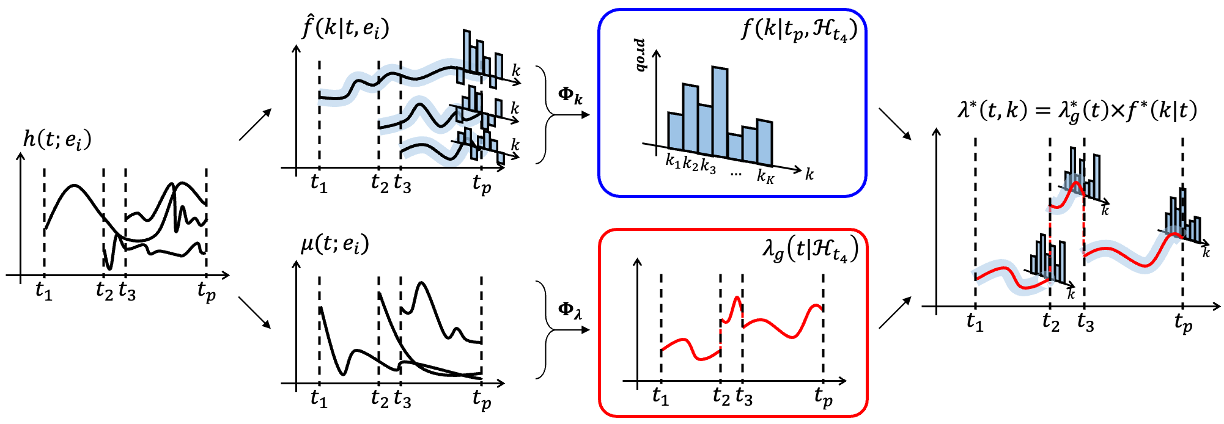
\includegraphics[width=0.95\linewidth]{figure/main_figure_final.png}
    \caption{\small A visualization of the overall framework. Hidden states from each event $e_i$ are independently propagated and decoded into trajectories of $\mu(t;e_i)$ and $\hat{f}_k (k|t, e_i)$. Each trajectory represents the effect of each event on the MTPP, and the MTPP can be reconstructed by combining all trajectories.}
    % \vspace{-10pt}
    \label{fig:main}
    % \vspace{-5pt}
\end{figure}

\section{Decoupling Marked Time Point Process}
Our approach focuses on establishing a general framework that captures the high-fidelity distribution of MTPP with decoupled structures. 
Specifically, given a sequence of events denoted as $\mathcal{S} = \{e_i\}_{i=0} ^n$
, where an event $e_i = (t_i, k_i)$ is composed of a time point and a marker, with $n+1$
observed events, our goal is to predict a probability distribution of an event $e_{n+1}$. 
Unlike previous works that directly estimate the conditional intensity $\lambda^*(t,k)$, we take an alternative approach of 
separately estimating the ground intensity and the distribution of event, i.e., $\lambda _g ^*(t)$ and $f^*(k|t)$. 

In our framework, the influences from each events through time are represented by hidden state dynamics $h(t;e_i)$, which  
undergo a decoding process 
to yield $\lambda ^*_g(t)$ and $f^*(k|t)$ separately. As described in Fig.\ref{fig:main}, $\lambda^* _g(t)$ and $f^*(k|t)$ form independent trajectories, and they are combined in the later stage to constitute $\lambda^*(t,k)$.


\subsection{Hidden State Dynamics \label{continuous modeling}} 

In this section, we introduce decoupled hidden state dynamics, 
where the hidden state is used to characterize the influence each event $e_i$ has on the overall process.

The decoupled hidden states $h(t; e_i) \in \mathbb{R}^d$, where $i=1, \cdots, n$,
are independently propagated through time from the occurrence of each event at $t_i$.  
The dynamics of $h(t; e_i)$, which will be used to characterize the complex dynamics of the intensity function within MTPP, are trained using the Neural ODEs \cite{bib:node}. 

Specifically, the initial magnitude of a hidden state $h(t_i;e_i)$ depends on the event type $k_i$, 
and the 
dynamics are solved via initial value problem (IVP) solvers. 
Then the hidden state caused by an event $e_i$ at time $t$ can be obtained as: 
\begin{align}
d h(t;e_i) &=  \gamma(h(t;e_i), t, k_i;\theta) dt \\
h(t;e_i) &= h(t_i;e_i) + \int ^t _{t_i} \gamma(h(s;e_i), s, k_i;\theta) ds \nonumber\\
& = W_{e}(k_i) + \int ^t _{t_i} \gamma(h(s;e_i), s, k_i;\theta) ds 
\label{eq:hiddenS}
\end{align}
where the initial magnitude is obtained using $W_{e}(\cdot): \{1, \cdots, K\} \rightarrow \mathbb{R}^{d}$, which is trainable, and $\gamma$ is parameterized with a neural network $\theta$. Hidden states at time $t$ can be computed in parallel as a multidimensional ODE by 
taking advantages of the decoupled structure of $h(t;e_i)$ as 
\begin{align}
    {d \over dt} \mathbf{h(t)} = 
    {d \over dt}
    \begin{bmatrix}
        h(t;e_0) \\
        \vdots \\ h(t;e_i)
    \end{bmatrix}
    = 
    \begin{bmatrix}
        \gamma(h(t;e_0), t, k_0;\theta) \\ \vdots \\ \gamma(h(t;e_i), t, k_i; \theta)
    \end{bmatrix}. 
    \label{eq: hidden parallel}
\end{align}
One major advantage of the decoupling is that the influence of events from $\mathbf{h}(t)$ can be selectively considered. 
For example, when computing $f^*(t)$ 
conditioned on $\mathcal{H}_{t_j}$, where $t > t_{j+1}$, $h(t;e_{t_{j+1}})$ should not be included in computation. The details will be discussed in the Sec. \ref{sec:ground int}.

\subsection{Ground intensity function \label{sec:ground int}}

In our method, the ground intensity $\lambda _g ^*(t)$ is defined as a mixture of decoupled \textit{influence functions} $\mu(t;e_i)$, which can be considered as a generalized form of the exciting functions found in the Hawkes process \cite{bib:hawkes}. 
Since each influence function is conditioned on a single event, in order to define $\lambda _g (t|\mathcal{H}_t)$, i.e., the ground intensity conditioned on the history, the influences from historical events must be aggregated. 
The conditional ground intensity function is defined as,
\begin{align}
    \lambda_g(t|\mathcal{H}_{t_{n+1}}) =\lambda_g(t|e_0, \cdots, e_n) = \Phi_\lambda(\mu(t;e_0), \cdots, \mu(t;e_n))
    \label{eq:lambdag}
\end{align}
where $\mu(t;e_i) := g_\mu(h(t;e_i))$ is decoded by a neural network $g_\mu : \mathbb{R}^d \rightarrow \mathbb{R}$, $ e_i \in \mathcal{H}_{t_{n+1}}$ is an observed event, and $\Phi_\lambda$ is a positive function to satisfy the non-negativity constraints of $\lambda ^* _g (t)$. 
Notice that the hidden state $h(t;e_i)$ is decoded into the influence function $\mu(t;e_i)$ before aggregated into $\lambda ^*_g(t)$, otherwise, influence from a specific event would not be observable. 



When learning a TPP, integration is pivotal. Not only does the computation of probability distribution $f ^*(t):= \lambda^*(t) \exp(-\int _{t_{i-1}} ^t \lambda^* (s) ds)$ requires an integration, but also obtaining characteristic functions, survival rate, etc. requires additional integration 
which does not have a closed-form solution in general. 
Therefore, intensity-based methods often require additional steps for predictions. 
Methods such as Monte Carlo Inference \cite{bib:nhp, bib:sahp, bib:THP, bib:ANHP} are often used for calculating $f^*(t)$, 
while sampling methods such as the thinning algorithm \cite{bib:nhp} are adopted for computing the expected value. 
In these approaches, each integration has to be handled separately with additional sampling.
The Neural ODEs, which we extensively utilize to solve for the MTPP, 
is inherently computationally heavier compared to Monte Carlo Inference due to its sequential solving mechanism. 
To circumvent the extra computational burden, we leverage the characteristics of the differential equation. 
By simultaneously solving the following multi-dimensional differential equation with respect to $\mathbf{h}(t)$ along with numerical integration, we eliminate the need for additional sampling: 
\begin{align}
\label{eqn:multi-integral}
{\partial \over \partial t} 
\begin{bmatrix}
\mathbf{h}(t) \\[1.5ex] 
\Lambda_g (t |  \mathcal{H}_{t_i}) \\[1.5ex] 
F(t | \mathcal{H}_{t_i}) \\[1.5ex] 
\mathbb{E}[t]
\end{bmatrix}
= 
\begin{bmatrix}
\gamma (\mathbf{h}(t),t, \mathbf{k}; \theta) \\[1.5ex] 
\lambda_g(t | \mathcal{H}_{t_i}) \\[1.5ex] 
f(t|\mathcal{H}_{t_i}) \\[1.5ex] 
t \cdot f(t|\mathcal{H}_{t_i})
\end{bmatrix}
= 
\begin{bmatrix}
\gamma (\mathbf{h}(t),t,\mathbf{k}; \theta) \\[1.5ex] 
\Phi_\lambda( g_\mu(\mathbf{h}(t))) \\[1.5ex] 
\lambda_g(t|\mathcal{H}_{t_i}) \cdot \exp (\Lambda_g(t_{i-1}|\mathcal{H}_{t_i}) - \Lambda_g(t|\mathcal{H}_{t_i}) ) \\[1.5ex] 
t \cdot f(t|\mathcal{H}_{t_i}) 
\end{bmatrix}
\end{align}

where $\Lambda_g (t|\mathcal{H}_{t_i}) := \int ^t _0 \lambda_g (t | \mathcal{H}_{t_i}) dt$ is called the \textit{compensator}, and $\mathbf{k}$ is the marks corresponding to $\mathbf{h}(t)$. Because the dynamics are learned through differential equations, values at time $t$ can be used for computing others. e.g., $\lambda^*_g(t)$, which is a derivative of $\Lambda^*_g(t)$, can be computed using $\mathbf{h}(t)$.

\begin{wrapfigure}{r}{0.52\textwidth}
% \vspace{-5pt}
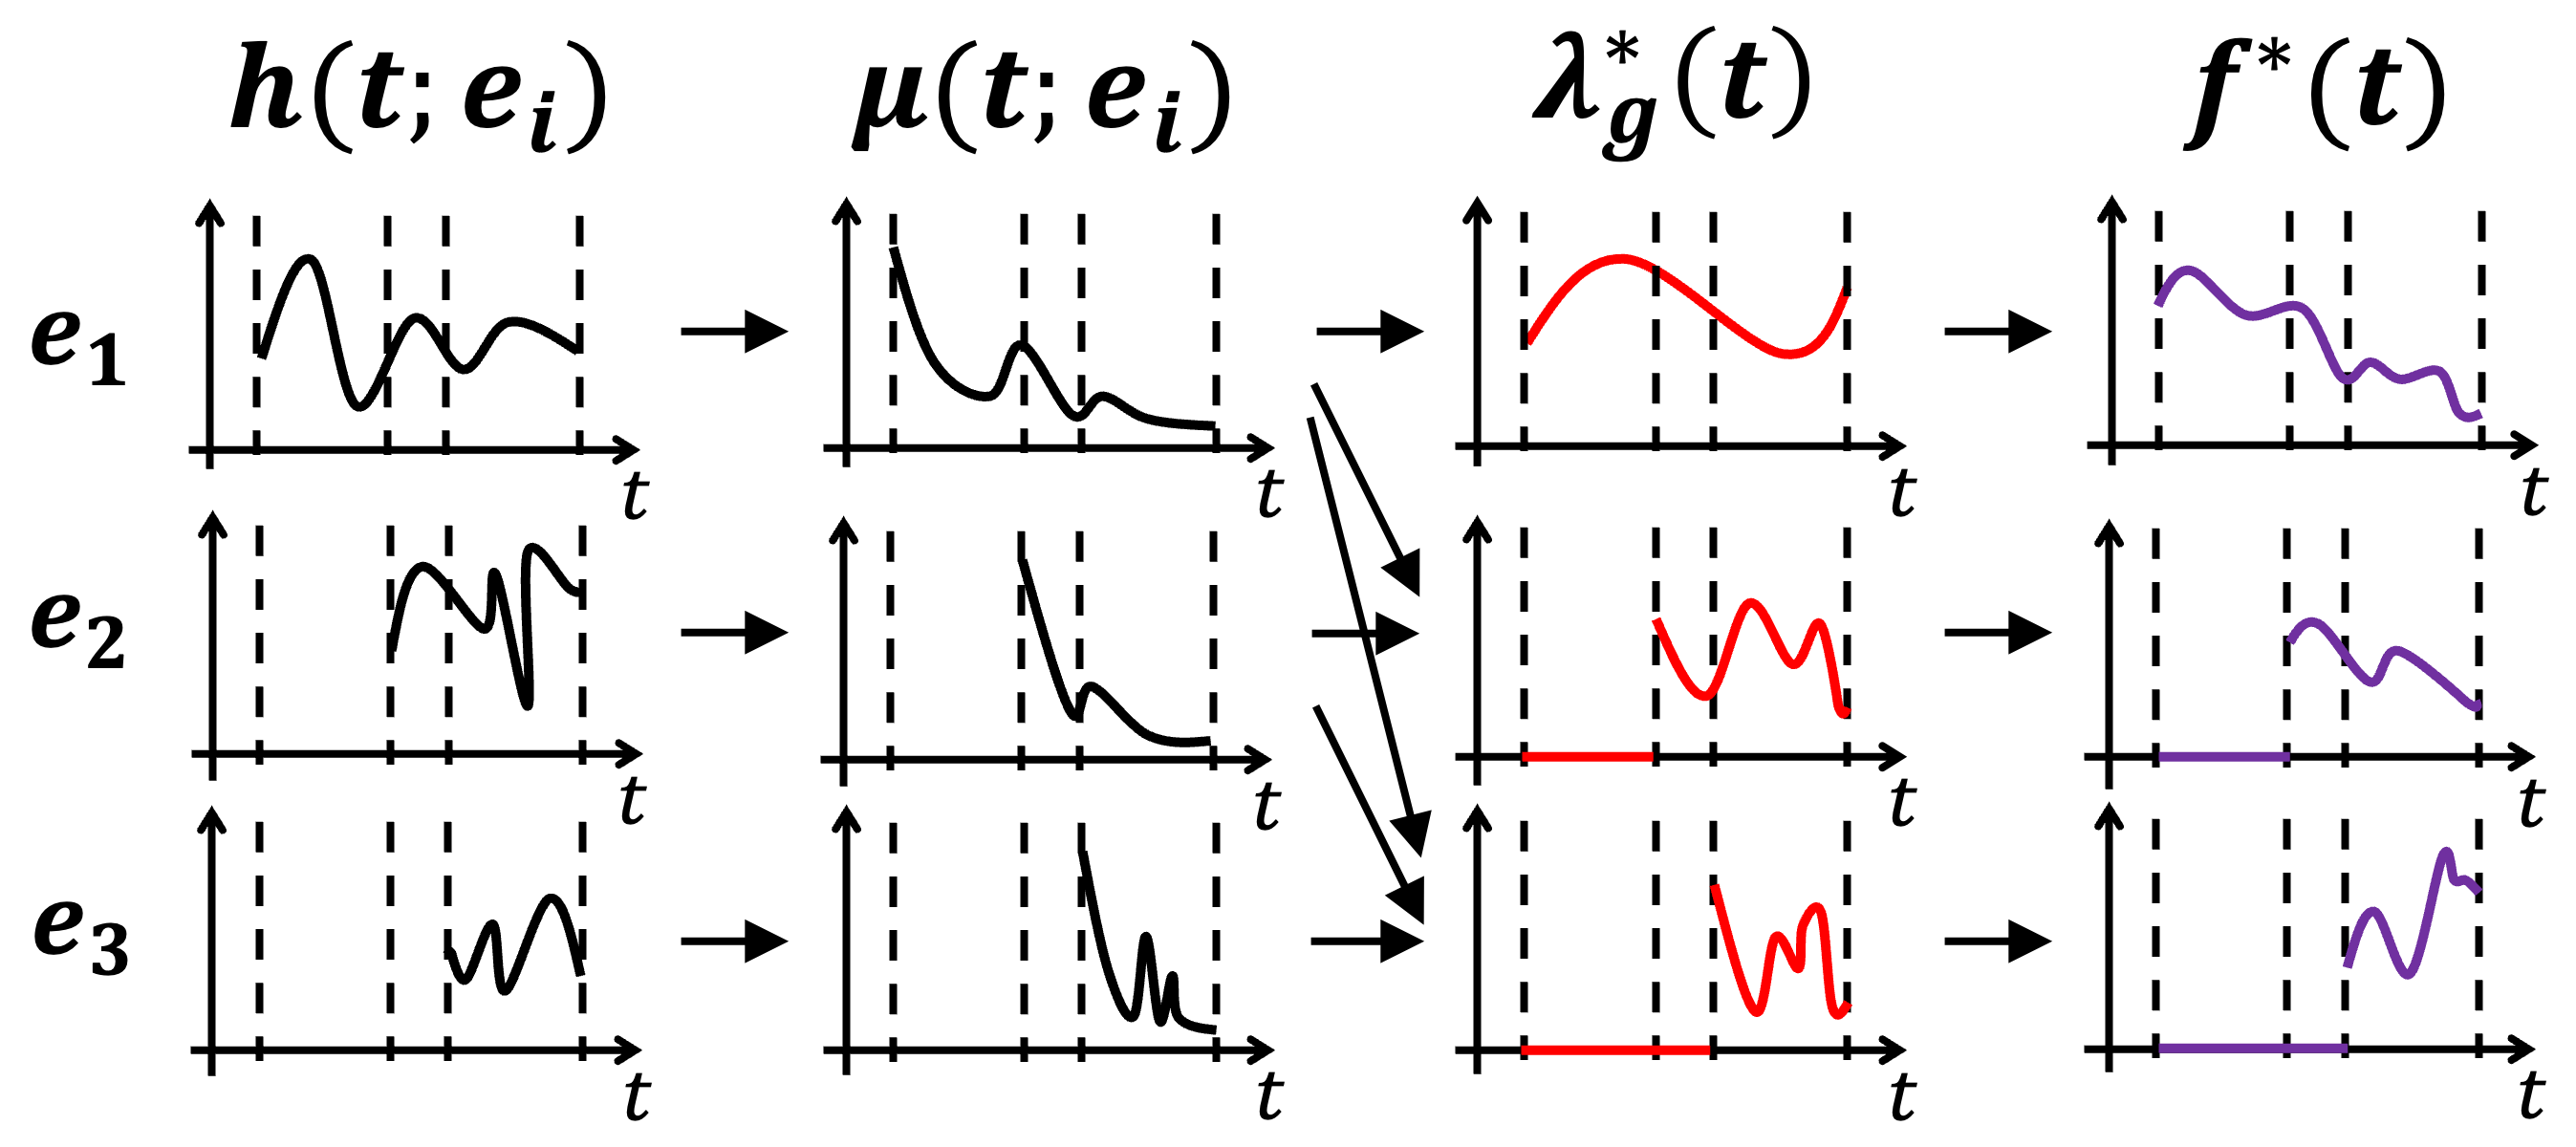
\includegraphics[width=0.50\textwidth]{figure/eq_9_figure2.png}
\captionsetup[figure]{font=small}
% \vspace{-3pt}
\caption{\small Visualization of \eqref{eqn:multi-integral}. Different combinations of $\mu(t;e_i)$ can be selected for calculating $\lambda ^*_g(t)$ and $f^*(t)$ conditioned on different $\mathcal{H}_{t_i}$ in parallel.}
% \vspace{-15pt}
\label{fig: selective DE}
\end{wrapfigure} 
Therefore, important estimations with integration, such as likelihood, survivor rate $S ^* (t) := 1- F^*(t)$, 
and $\mathbb{E}_{f^*} [t]$ can be predicted in a single run. 
This formulation can be applied to any number of integrations.
Moreover, as briefly mentioned in Sec. \ref{continuous modeling}, the influence functions can be selected according to our interests as illustrated in Fig. \ref{fig: selective DE}. 
Therefore, approximations of functions in \eqref{eqn:multi-integral} under different $\mathcal{H}_{t_i}$ can be obtained in parallel, distinguishing Dec-ODE from other intensity-based methods that require separate runs. 

% \vspace{-5pt}
\subsection{Conditional Probability for Marks \label{sec:fk}}
% \vspace{-5pt}

Similar to the formulation of the ground intensity in \eqref{eq:lambdag}, the probability of marks $f^* (k|t)$ can be expressed using the following form: 
\begin{equation}
 f(k|t, \mathcal{H}_{t_{n+1}}) = \Phi _k( \hat{f}(k|t,e_0), \cdots, \hat{f}(k|t,e_{n}))
 \end{equation}
where $\hat{f}(k|t,e_i):= g_f(h_t(e_i))$ is an influence from $e_i$ on $f(k|t)$, decoded by a neural network $g_f(\cdot)$. The function $\Phi_k$ combines $\hat{f}(k|t,e_i)$ over events while satisfying $\sum _K \Phi_k(\cdot)  = 1$. 

The intuition behind such a modeling is that the context of an event changing over time carries important information. For instance, getting a driver's license would dramatically increase the probability of causing a car accident since there was no chance without the license. 
However, as time goes on, the person gets better at driving and the probability decreases. 
Using the proposed structure, the changes of implications through time can be inferred by $\hat{f}(k|t_i,e_i)$.

 
\section{Linear Dec-ODE \label{Linear Decode}}

The combining functions $\Phi_\lambda$ and $\Phi_k$ can be chosen from a simple summation to a complex neural networks, such as Transformer. 
Nonetheless, in the following section, we present 
a linear version of Dec-ODE as it offers efficiency and interpretability via parallel modeling of the hidden states. 


\subsection{Combining Influences from Past Events}
In order to demonstrate the competence of the proposed framework, the implementation of $\Phi_\lambda$ and $\Phi_k$ is defined as linear and simple equations that combines influences of historical events for $\lambda ^* _g(t)$ and $f^*(k|t)$. 
The ground intensity $\lambda^* _g (t)$ and the conditioned probability of marks $f^*(k|t)$ are defined as combinations of decoupled dynamics :
\begin{equation}
\begin{aligned}
\lambda _g (t| \mathcal{H}_{t_{n+1}}) = \Phi_\lambda(\mu(t;e_0), \cdots, \mu(t;e_n)) = \sum _{e_i \in \mathcal{H}_{t_{n+1}}} \text{softplus} (\mu  (t; e_i))
\end{aligned}
\label{eq: lin-ground}
\end{equation}
\begin{equation}
\begin{aligned}
f(k|t, \mathcal{H}_{t_{n+1}}) = \Phi _k( \hat{f}(k|t,e_0), \cdots, \hat{f}(k|t,e_n)) = \text{softmax} \bigg( \sum_{e_i \in \mathcal{H}_{t_{n+1}}} \hat{f}(k|t,e_i)\bigg)
\end{aligned}
\end{equation}
where softplus and softmax functions are used to satisfy the constraints from Sec. \ref{sec:ground int} and Sec. \ref{sec:fk}, respectively.
This modeling of $\lambda^*_g(t)$ with linear summation resembles with the Hawkes process. 
Yet, our method can model more flexible temporal dynamics, and better suited for modeling complex real-life scenarios. 
 
%  \vspace{-5pt}
\subsection{Training Objective \label{sec:obj}}
% \vspace{-5pt}
The objective of our method is to maximize the likelihood of the predicted Marked TPP \cite{bib:daley}. 
Taking a $\log$ on the likelihood in \eqref{eq:likelihood}, 
\begin{equation}
\begin{aligned}
\ln f(t,k) &= \ln  \bigg[\prod ^{\mathcal{N}_g(t_N)} _{i=1} \lambda ^* _g (t_i)\bigg]\bigg[\prod ^{\mathcal{N}_g(t_N)} _{i=1} f ^* (k_i | t_i) \bigg] \exp \bigg( - \int ^{t_N} _0 \lambda ^*_g (u) du \bigg) \\
 &= \underbrace{\sum ^{\mathcal{N}_g(t_N)} _{i=1} \ln \lambda ^* _g (t_i) -   \int ^{t_N} _0 \lambda ^*_g (u) du}_{\ln L_\lambda} + \underbrace{\sum ^{\mathcal{N}_g(t_N)} _{i=1} \ln f ^* (k_i | t_i)}_{\ln L_k}
\label{eq:obj}
\end{aligned}
\end{equation}
where $t_N$ is the last observed time point, and the log-likelihood for the ground intensity $\ln L_\lambda$ and the mark distribution $\ln L_k$ are independently defined,
and used to learn $\lambda_g(t)$ and $f(k|t)$, respectively.
Intuitively, the first term in $L_\lambda$ is the probability of event happening at each $t_i$ and the second term is the probability of event not happening everywhere else. 
Therefore, $\lambda^*_g(t)$ should be high at the time of event's occurrence and low everywhere else to maximize $L_\lambda$.
Also, for the estimations, $f(t)$ is normalized to satisfy $\int f(t) dt = 1$.

% \vspace{-5pt}
\subsection{Training Scheme \label{train_parallel}}
% \vspace{-5pt}
Many previous works using differential equation based modeling \cite{bib:NJSDE, bib:STPP} 
sequentially solve the entire time range, which require  
exhaustive training time. 
In our case, using the characteristics of $\Phi_\lambda$ with linear summation, such limitation can be alleviated as follows. 

First, because each $\mu(t; e_i)$ is independent from other events, we can propagate them simultaneously as a multi-dimensional differential equation as
\begin{equation}
    d 
    \begin{bmatrix}
        \mu(\tau_0 ;e_0) \\ \vdots \\ \mu(\tau_i;e_i)
    \end{bmatrix}
    = 
    \begin{bmatrix}
        \gamma(\mu(\tau_0), \tau_0, k_0;\theta) \\ \vdots \\ \gamma(\mu(\tau_i), \tau_i, k_i; \theta)
    \end{bmatrix}
    \cdot d \boldsymbol{\tau}
    \label{eq: train_parallel}
\end{equation}
where $ \boldsymbol{\tau} =[\tau_0, \cdots, \tau_i] ^\top = [t_0 + t, t_1 + t, \cdots, t_i + t] ^ \top$. 

Second, one of the benefits of formulating the ground intensity as a linear equation is that 
the compensator $\Lambda^* _g(t)$ can also be calculated in the same manner as in \eqref{eq: lin-ground}
\begin{align}
    \Lambda^* _g (t)  & = \int _0 ^t \lambda_g ^* (s) ds = \int_0 ^t \sum _{e_i \in \mathcal{H}_{t}} \text{softplus} (\mu  (s; e_i)) ds \\    
    & = \sum_{e_i \in \mathcal{H}_{t}} \int _{t_i} ^t \text{softplus}( \mu (s; e_i)) ds
    \label{eq:Lambda}
\end{align}
where the region of the integration changes since there is no influence of $e_i$ before $t_i$.
The \eqref{eq:Lambda} conveys that the integration in \eqref{eq:obj} can be computed by integrating softplus
$(\mu(t;e_i))$ individually first and sum up later, 
instead of sequentially going through the entire sequence. 
Hence, if we can find the number of time-points $m$, we can solve the entire trajectory within a fixed number of steps. The effectiveness of such modeling is discussed in Sec. \ref{ablation: parallel}.
\begin{figure}[h]
    \centering
    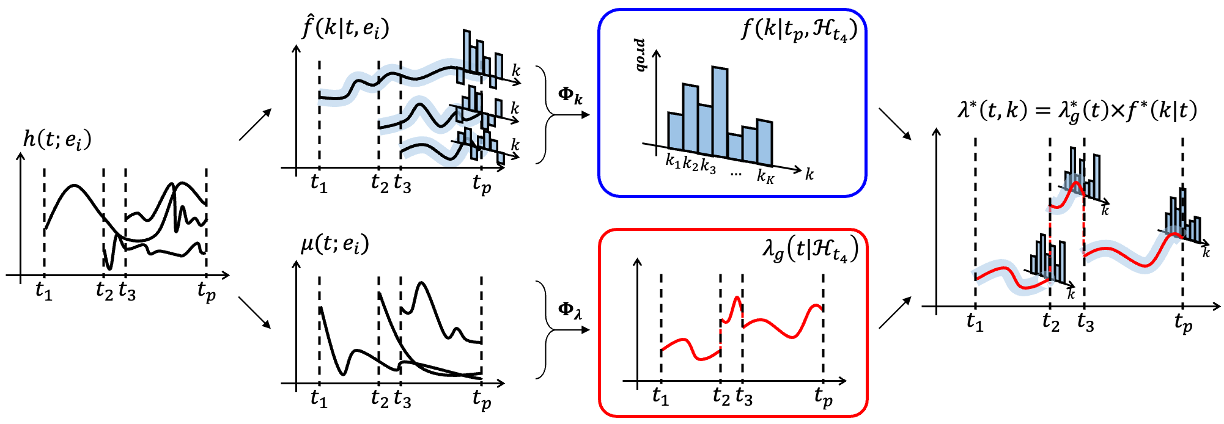
\includegraphics[width=0.95\linewidth]{figure/main_figure_final.png}
    \caption{\small Overview of the proposed framework. Hidden states corresponding to each event $e_i$ are individually propagated and decoded into trajectories $\mu(t;e_i)$ and $\hat{f}_k (k|t, e_i)$. These trajectories represent the influence of individual events on the MTPP, which is reconstructed by aggregating all the trajectories.}
    \label{fig:main}
\end{figure}

\section{Decoupling Marked Temporal Point Processes}
This work introduces a generalizable framework designed to effectively model MTPP distributions through decoupled structures. 
For a sequence of events $\mathcal{S} = \{e_i\}_{i=0} ^n$, where each event $e_i = (t_i, k_i)$ consists of a timestamp $t_i$ and a marker $k_i$, the objective is to predict the distribution of the next event $e_{n+1}$. 
Rather than directly estimating the conditional intensity $\lambda^*(t,k)$ as in prior approaches, we adopt a decoupled modeling strategy by separately estimating the ground intensity $\lambda^*_g(t)$ and the event distribution $f^*(k|t)$.

In our framework, the temporal influence of each event is captured by hidden state dynamics $h(t;e_i)$, which are decoded to yield $\lambda^*_g(t)$ and $f^*(k|t)$. As shown in Fig.~\ref{fig:main}, these two components are modeled as separate trajectories and are combined to recover $\lambda^*(t,k)$.

\subsection{Hidden State Dynamics \label{continuous modeling}}

The framework incorporates hidden state dynamics that are decoupled for each event. These hidden states characterize the impact of an event $e_i$ on the overall process.
The decoupled hidden states, $h(t; e_i) \in \mathbb{R}^d$ for $i = 1, \cdots, n$, evolve independently over time from the occurrence of each event at $t_i$. These dynamics are parameterized using Neural ODEs~\cite{bib:node} to model the intricate behavior of the intensity function in MTPP.

The initial state $h(t_i;e_i)$ depends on the event type $k_i$, and the dynamics are computed by solving an initial value problem (IVP). The hidden state for event $e_i$ at time $t$ is given as:
\begin{align}
d h(t;e_i) &=  \gamma(h(t;e_i), t, k_i;\theta) dt, \\
h(t;e_i) &= h(t_i;e_i) + \int_{t_i}^t \gamma(h(s;e_i), s, k_i;\theta) ds \nonumber \\
&= W_{e}(k_i) + \int_{t_i}^t \gamma(h(s;e_i), s, k_i;\theta) ds,
\label{eq:hiddenS}
\end{align}
where $W_e(\cdot): \{1, \cdots, K\} \rightarrow \mathbb{R}^d$ is a trainable embedding, and $\gamma$ is a neural network parameterized by $\theta$. Since $h(t;e_i)$ is decoupled, hidden states at time $t$ can be computed in parallel as a multidimensional ODE:
\begin{align}
    \frac{d}{dt} \mathbf{h}(t) = 
    \frac{d}{dt}
    \begin{bmatrix}
        h(t;e_0) \\
        \vdots \\ 
        h(t;e_i)
    \end{bmatrix}
    = 
    \begin{bmatrix}
        \gamma(h(t;e_0), t, k_0;\theta) \\ 
        \vdots \\ 
        \gamma(h(t;e_i), t, k_i;\theta)
    \end{bmatrix}.
    \label{eq:hidden_parallel}
\end{align}

The decoupled structure enables selective use of hidden states when computing $f^*(t)$ under specific histories $\mathcal{H}_t$, such as omitting $h(t;e_{j+1})$ when $t > t_{j+1}$. Detailed usage is described in Sec.~\ref{sec:ground int}.

\subsection{Ground Intensity Function \label{sec:ground int}}

The ground intensity $\lambda^*_g(t)$ is modeled as a combination of event-specific \textit{influence functions} $\mu(t;e_i)$, which generalize the excitation functions in Hawkes processes~\cite{bib:hawkes}. To compute $\lambda_g(t|\mathcal{H}_t)$, the influences of historical events are aggregated:
\begin{align}
    \lambda_g(t|\mathcal{H}_{t_{n+1}}) = \Phi_\lambda(\mu(t;e_0), \cdots, \mu(t;e_n)),
    \label{eq:lambdag}
\end{align}
where $\mu(t;e_i) := g_\mu(h(t;e_i))$, decoded via a neural network $g_\mu: \mathbb{R}^d \rightarrow \mathbb{R}$. The aggregation function $\Phi_\lambda$ ensures non-negativity. Decoding $\mu(t;e_i)$ prior to aggregation ensures visibility of individual event influences.

\subsection{Integration and Prediction via Neural ODEs}

The computation of various quantities such as likelihood, survival rates, and expected values in MTPP necessitates integration. Neural ODEs, being computationally demanding due to sequential solvers, are leveraged efficiently by solving multi-dimensional differential equations:
\begin{align}
\label{eqn:multi-integral}
{\partial \over \partial t} 
\begin{bmatrix}
\mathbf{h}(t) \\[1.5ex] 
\Lambda_g (t |  \mathcal{H}_{t_i}) \\[1.5ex] 
F(t | \mathcal{H}_{t_i}) \\[1.5ex] 
\mathbb{E}[t]
\end{bmatrix}
= 
\begin{bmatrix}
\gamma (\mathbf{h}(t),t, \mathbf{k}; \theta) \\[1.5ex] 
\lambda_g(t | \mathcal{H}_{t_i}) \\[1.5ex] 
f(t|\mathcal{H}_{t_i}) \\[1.5ex] 
t \cdot f(t|\mathcal{H}_{t_i})
\end{bmatrix}
= 
\begin{bmatrix}
\gamma (\mathbf{h}(t),t,\mathbf{k}; \theta) \\[1.5ex] 
\Phi_\lambda( g_\mu(\mathbf{h}(t))) \\[1.5ex] 
\lambda_g(t|\mathcal{H}_{t_i}) \cdot \exp (\Lambda_g(t_{i-1}|\mathcal{H}_{t_i}) - \Lambda_g(t|\mathcal{H}_{t_i}) ) \\[1.5ex] 
t \cdot f(t|\mathcal{H}_{t_i}) 
\end{bmatrix}
\end{align}

This eliminates the need for separate integration steps, enabling simultaneous computation of multiple quantities, as visualized in Fig.~\ref{fig: selective DE}.
Therefore, important estimations with integration, such as likelihood, survivor rate $S ^* (t) := 1- F^*(t)$, and $\mathbb{E}_{f^*} [t]$ can be predicted in a single run. 
This formulation can be applied to any number of integrations.

\begin{wrapfigure}{r}{0.44\textwidth}
    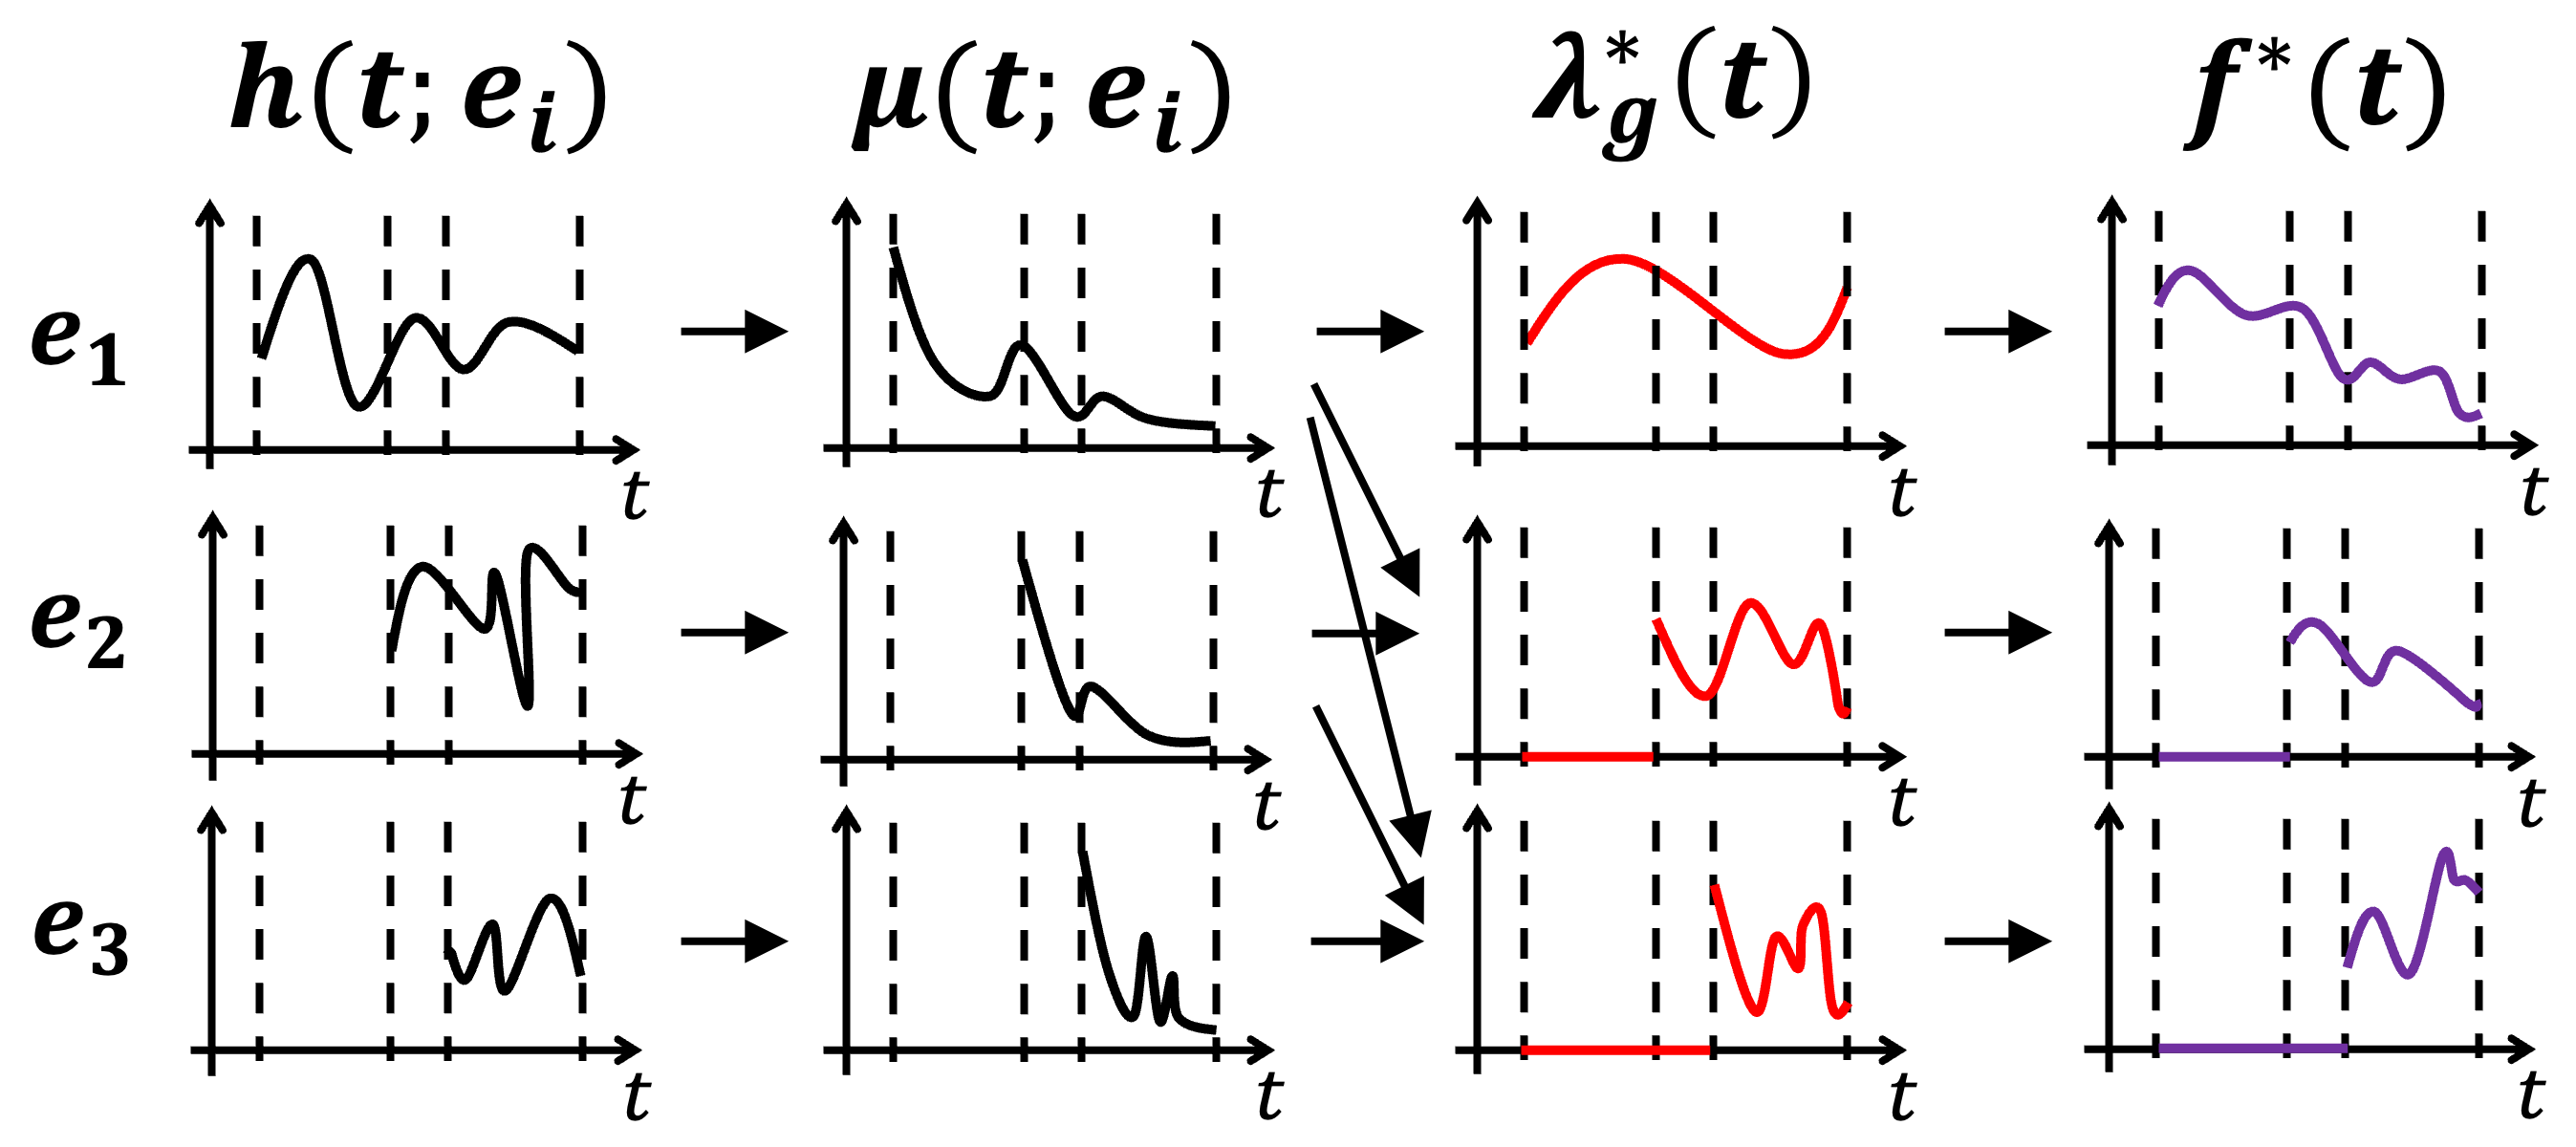
\includegraphics[width=0.42\textwidth]{figure/eq_9_figure2.png}
    \captionsetup[figure]{font=small}
    \caption{\small Visualization of \eqref{eqn:multi-integral}. Different combinations of $\mu(t;e_i)$ can be selected for calculating $\lambda ^*_g(t)$ and $f^*(t)$ conditioned on different $\mathcal{H}_{t_i}$ in parallel.}
    \label{fig: selective DE}
\end{wrapfigure} 
Moreover, as briefly mentioned in Sec. \ref{continuous modeling}, the influence functions can be selected according to our interests as illustrated in Fig. \ref{fig: selective DE}. 
Therefore, approximations of functions in \eqref{eqn:multi-integral} under different $\mathcal{H}_{t_i}$ can be obtained in parallel, distinguishing Dec-ODE from other intensity-based methods that require separate runs. 


\subsection{Conditional Probability for Marks \label{sec:fk}}

The conditional probability of marks $f^*(k|t)$ is formulated as:
\begin{equation}
 f(k|t, \mathcal{H}_{t_{n+1}}) = \Phi_k(\hat{f}(k|t,e_0), \cdots, \hat{f}(k|t,e_n)),
\end{equation}
where $\hat{f}(k|t,e_i):= g_f(h(t;e_i))$ and $\Phi_k$ ensures $\sum_K \Phi_k(\cdot) = 1$. This approach captures temporal dynamics in the event context, such as changing probabilities over time.

\section{Linear Dec-ODE}
\subsection{Combining Influences from Past Events}
To demonstrate the proposed framework's effectiveness, we implement a linear variant of Dec-ODE. Here, $\Phi_\lambda$ and $\Phi_k$ are defined as simple linear combinations while satisfying the constraints using activation functions:
\begin{align}
\lambda_g(t|\mathcal{H}_{t_{n+1}}) &= \sum_{e_i \in \mathcal{H}_{t_{n+1}}} \text{softplus}(\mu(t;e_i)), \label{eq: lin-ground}\\
f(k|t, \mathcal{H}_{t_{n+1}}) &= \text{softmax}\left(\sum_{e_i \in \mathcal{H}_{t_{n+1}}} \hat{f}(k|t,e_i)\right).
\end{align}

The linearity offers interpretability and scalability while supporting complex temporal dynamics beyond classical Hawkes processes. 

\subsection{Training Objective \label{sec:obj}}

The goal of our approach is to maximize the likelihood of the predicted Marked TPP \cite{bib:daley}. Taking the logarithm of the likelihood in \eqref{eq:likelihood}, we obtain:
\begin{equation}
\begin{aligned}
\ln f(t, k) &= \ln \bigg[\prod^{\mathcal{N}_g(t_N)}_{i=1} \lambda^*_g(t_i)\bigg] \bigg[\prod^{\mathcal{N}_g(t_N)}_{i=1} f^*(k_i | t_i) \bigg] \exp\bigg(- \int_0^{t_N} \lambda^*_g(u) du \bigg) \\
 &= \underbrace{\sum^{\mathcal{N}_g(t_N)}_{i=1} \ln \lambda^*_g(t_i) - \int_0^{t_N} \lambda^*_g(u) du}_{\ln L_\lambda} + \underbrace{\sum^{\mathcal{N}_g(t_N)}_{i=1} \ln f^*(k_i | t_i)}_{\ln L_k},
\label{eq:obj}
\end{aligned}
\end{equation}
where $t_N$ is the final observed time point. The log-likelihood terms $\ln L_\lambda$ for the ground intensity and $\ln L_k$ for the mark distribution are defined separately and are used to learn $\lambda_g(t)$ and $f(k | t)$, respectively.

Conceptually, the first term in $L_\lambda$ captures the likelihood of events occurring at each $t_i$, while the second term accounts for the likelihood of events not occurring at all other times. To maximize $L_\lambda$, $\lambda^*_g(t)$ should be high at event occurrence times and low otherwise. 
Additionally, for estimation purposes, $f(t)$ is normalized to satisfy $\int f(t) dt = 1$.

\subsection{Training Scheme \label{train_parallel}}
% \vspace{-5pt}
Prior works leveraging differential equation-based modeling \cite{bib:NJSDE, bib:STPP} typically solve over the entire time range sequentially, resulting in substantial training time. In contrast, our approach mitigates this limitation by utilizing the properties of $\Phi_\lambda$ with linear summation, as described below.

First, since each $\mu(t; e_i)$ evolves independently of other events, they can be propagated simultaneously by solving a multi-dimensional differential equation:
\begin{equation}
    d 
    \begin{bmatrix}
        \mu(\tau_0 ;e_0) \\ \vdots \\ \mu(\tau_i;e_i)
    \end{bmatrix}
    = 
    \begin{bmatrix}
        \gamma(\mu(\tau_0), \tau_0, k_0;\theta) \\ \vdots \\ \gamma(\mu(\tau_i), \tau_i, k_i; \theta)
    \end{bmatrix}
    \cdot d \boldsymbol{\tau},
    \label{eq: train_parallel}
\end{equation}
where $ \boldsymbol{\tau} =[\tau_0, \cdots, \tau_i]^\top = [t_0 + t, t_1 + t, \cdots, t_i + t]^\top$. 

Second, formulating the ground intensity as a linear equation offers the advantage of computing the compensator $\Lambda^*_g(t)$ in a similar manner to \eqref{eq: lin-ground}:
\begin{align}
    \Lambda^*_g(t) & = \int_0^t \lambda_g^*(s) ds = \int_0^t \sum_{e_i \in \mathcal{H}_{t}} \text{softplus}(\mu(s; e_i)) ds \\    
    & = \sum_{e_i \in \mathcal{H}_{t}} \int_{t_i}^t \text{softplus}(\mu(s; e_i)) ds,
    \label{eq:Lambda}
\end{align}
where the integration bounds shift because the influence of $e_i$ begins only after $t_i$. 

Equation \eqref{eq:Lambda} illustrates that the integration in \eqref{eq:obj} can be performed by independently integrating $\text{softplus}(\mu(t; e_i))$ for each event and subsequently summing the results, rather than sequentially processing the entire sequence. Consequently, given a fixed number of time points $m$, the full trajectory can be solved in a fixed number of steps. The efficiency of this approach is further discussed in Sec. \ref{ablation: parallel}.


\chapter{Related Works}
% \section {Intensity modeling} 
When modeling TPP, tdhe intensity function is widely used due to its flexibility in capturing temporal distributions, and 
deep learning facilitated the parameterization of complex processes using neural networks. 
Initially, many focused on relaxing constraints of traditional TPP \cite{bib:hawkesOrigin, ISHAM1979335, bib:daley} such as Hawkes process. 
RNN based neural TPP models \cite{bib:nhp, bib:RMTPP} used RNNs to effectively encapsulate sequences into a history vector. 
Transformer-based methods \cite{bib:THP, bib:sahp} were used to encapsulate $\mathcal{H}_t$ while considering long term and short term dependency of events, and 
%Another variant of Transformer-based model the 
Attentive Neural Hawkes Process (ANHP) \cite{bib:ANHP} utilized self-attention for modeling complex continuous temporal dynamics by using a attention network on an unobserved event. 
\cite{bib:nonparam} used the Gaussian process to relax the exponential decaying effect of Hawkes process. 
\cite{bib:fully_neural} adopted a compensator function, which is a integration of an intensity function, to model TPP to alleviate computing issues in integration with no closed form. 

\section{Direct estimation of pdf} 
An alternative approach, which is to directly predicting the pdf of a TPP, has also been studied. \cite{bib:ifl} proposed a method to model the temporal distribution using a log-normal mixture. 
Having a closed form pdf allowed direct inference of important characteristics, 
while the mixture model provided flexible modeling. 
There exists various other methods that model the pdf directly using popular deep learning models including GAN, normalizing flow, variational auto encoder and meta learning \cite{bib:exploring_generative, bib:MetaTPP}.

\section{Learning temporal dynamics using Neural ODEs} 
In \cite{bib:node}, Neural ODE was proposed where the changes of hidden vector between layers are considered in a continuous manner. 
Differential equation based methods were incorporated into various temporal dynamic modeling \cite{bib:neuralTemporalWalk,bib:counterfactualCDE,bib:SDEGames}, showing advantages in modeling sparse and irregular time series.
\cite{bib:NJSDE} modeled the jump stochastic differential equation using Neural ODEs, and tested on TPP modeling. 
\cite{bib:STPP} expanded the work to modeling spatio-temporal point process and predicted both temporal and spatial dynamics using Neural ODEs and continuous normalizing flow. Also, an algorithm for handling time varying sequence in batch wise computation was proposed.
\section{Intensity Modeling} 
The intensity function is widely used in TPP modeling due to its flexibility in capturing temporal distributions, with deep learning enabling the parameterization of complex processes through neural networks. 
Early research often focused on relaxing the constraints of traditional TPPs such as the Hawkes process \cite{bib:hawkesOrigin, ISHAM1979335, bib:daley}. 
RNN-based neural TPP models \cite{bib:nhp, bib:RMTPP} leveraged RNNs to effectively encode event sequences into a history vector. 
Transformer-based approaches \cite{bib:THP, bib:sahp} accounted for both long-term and short-term event dependencies in $\mathcal{H}_t$. 
The Attentive Neural Hawkes Process (ANHP) \cite{bib:ANHP} further incorporated self-attention to model complex continuous temporal dynamics by applying attention mechanisms on unobserved events. 
In another direction, \cite{bib:nonparam} utilized Gaussian processes to relax the exponential decay assumption in the Hawkes process. 
Additionally, \cite{bib:fully_neural} proposed using a compensator function—an integral of the intensity function—to alleviate computational challenges associated with integration in the absence of a closed form.

\section{Direct Estimation of the PDF} 
Another approach involves directly predicting the probability density function (PDF) of a TPP. 
For instance, \cite{bib:ifl} proposed modeling the temporal distribution using a log-normal mixture. 
The closed-form PDF provided by this method enables direct inference of key characteristics, while the mixture model offers flexible modeling capabilities. 
Other approaches to modeling the PDF directly have incorporated popular deep learning frameworks such as GANs, normalizing flows, variational autoencoders, and meta-learning \cite{bib:exploring_generative, bib:MetaTPP}.

\section{Learning Temporal Dynamics with Neural ODEs} 
Neural ODEs, introduced in \cite{bib:node}, treat changes in the hidden vector between layers as continuous, offering a novel framework for modeling temporal dynamics. 
Differential equation-based methods have since been applied to a range of temporal dynamic modeling tasks \cite{bib:neuralTemporalWalk, bib:counterfactualCDE, bib:SDEGames}, demonstrating advantages in handling sparse and irregular time series. 
For instance, \cite{bib:NJSDE} used Neural ODEs to model jump stochastic differential equations and tested this on TPP modeling. 
\cite{bib:STPP} extended this work to spatio-temporal point processes, predicting both temporal and spatial dynamics using Neural ODEs and continuous normalizing flows, and proposed a batch-wise computation algorithm for time-varying sequences.


\chapter{Experiment}
% 
\section{Comparison on benchmarks}
In this section we compare linear Dec-ODE with the state-of-the-art methods using conventional benchmarks. 
\subsection{Experiment Setup \label{sec:experimentSetup}}
\label{sec:setup}
\textbf{Datasets.} 
We used five popular real-world datasets %that are 
from various domains: 
{\bf Reddit} is a sequences of social media posts, 
{\bf Stack Overflow (SO)} is a sequences of rewards received from the question-answering platform, 
{\bf MIMIC-II} is a sequences of diagnosis from Intensive Care Unit (ICU) clinical visits, 
{\bf MOOC} is a sequence of user interactions with the online course,
and {\bf Retweet} is also a sequences of social media posts. See Appendix for detailed description of these datasets. 
To obtain the results in a comparable scale, all time points were scaled down with the standard deviation of time gaps, $\{t_i - t_{i-1}\}_{i=1} ^n$, of the training set similar to \cite{bib:MetaTPP}. 

\textbf{Metrics.} 
We used three conventional metrics for the evaluation: 
1) \textit{negative log-likelihood} (NLL) validates the feasibility of the predicted probability density which is calculated via \eqref{eq:obj}, 2) \textit{root mean squared error} (RMSE) measures the reliability of the predicted time points of events,  
3) \textit{accuracy} (ACC) measures the correctness of the mark distribution $f^*(k|t)$. 
For the prediction, the expected value $\mathbb{E}_{f^*} [t]$ was used as the next arrival time of an event, 
and the mark with the highest probability at time $t$, i.e., $\argmax(f^*(k|t))$, was used as the predicted mark.

\textbf{Baseline.} We compared our methods with three state-of-the-art methods: 
Transformer Hawkes Process (THP) \cite{bib:THP}, Intensity-Free Learning (IFL) \cite{bib:ifl}, and Attentive Neural Hawkes Process (ANHP) \cite{bib:ANHP}. 
As THP and ANHP are both transformer-based methods, they  
effectively leverage the entire observed events $\mathcal{H}_{t_{n}}$ for predicting $e_{n+1}$.
IFL directly predicts $f^*(t,k) = f^*(t) f^*(k|t)$ using a log-normal mixture to predict a flexible distribution. 
Since it parameterizes the distribution $f^*(t)$, $\mathbb{E}_{f^*}[t]$ can be obtained in a closed form.
More details about the implementation are in Sec.\ref{sec:baselineImplementation}.

\begin{table}[!t]
\centering
\caption{Comparison with the state of the art methods on 5 popular real-life datasets. Results with \textbf{boldface} and \underline{underline} represent the best and the second-best results, respectively. Following \cite{bib:THP, bib:ANHP} the mean and std are gained by bootstrapping 1000 times.}
\renewcommand{\arraystretch}{1.3}
\small
\scalebox{0.52}[0.52]{

\begin{tabular}{c | c c c c | c | c c c c | c | c c c c | c} 
& \multicolumn{5}{c|}{RMSE} & \multicolumn{5}{c|}{ACC} & \multicolumn{5}{c}{NLL}\\
\cline{2-6} \cline{7-11} \cline{12-16}
&  RMTPP & THP & IFL & ANHP & \textbf{Dec-ODE} & RMTPP & THP & IFL & ANHP & \textbf{Dec-ODE} & RMTPP & THP & IFL & ANHP & \textbf{Dec-ODE}\\ 
\hline
\hline
\multirow{2}{*}{MOOC} & $0.473$ & $0.476$ & $0.501$ & \underline{$0.470$} & $\textbf{0.467}$
                        & $20.98$ & $24.49$ & $\underline{32.30}$ & $31.53$ & $\textbf{42.08}$ 
                        & $-0.315$ & $0.733$ & $\textbf{-2.895}$ & $\underline{-2.632}$ & $-2.289$  \\  [-3pt]
                    & ${(0.012)}$ & $(0.010)$ & ${(0.012)}$ & $\underline{(0.019)}$ & $\textbf{(0.012)}$
                    & $(0.29)$ &${(0.22)}$ & $\underline{(1.30)}$ & $(0.20)$ & $\textbf{(0.44)}$
                    & $(0.031)$ & $(0.047)$ & $\textbf{(0.031)}$ & $(\underline{0.043})$ & ${(0.191)}$ \\[3pt]
\multirow{2}{*}{Reddit} & $\underline{0.953} $ & $6.151$ & $1.040$ & $1.149$ & $\textbf{0.934}$
                        & $29.67$ & $60.72$ & $48.91$ & $\textbf{63.45}$ & $\underline{62.32}$ 
                        & $3.559$ & $2.335$ & $2.188$ & $\textbf{1.203}$ & $\underline{1.367}$ \\[-3pt]
                        & $\underline{(0.016)}$ & $(0.195)$ &  $(0.017)$ & $(0.010)$ & $\textbf{(0.017)}$
                        & $(1.19)$ & $(0.08)$ & $(1.27)$ & $\textbf{(0.16)}$ & $\underline{(0.11)}$ 
                        & $(0.070)$ &$(0.031)$ & $(0.088)$ & $\textbf{(0.068)}$ & $\underline{(0.126)}$ \\[3pt]
\multirow{2}{*}{Retweet} & $\underline{0.990} $ & $1.055$ & $1.012$ & $1.663$ & $\textbf{0.985}$ 
                        & $51.72$ & $\textbf{60.68} $ & $55.35$ & ${59.72}$ & $\underline{60.17}$ 
                        & $-2.180$ & $-2.597$ & $-2.672$ & $\textbf{-3.134}$ & $\underline{-2.897}$ \\[-3pt]
                    & $\underline{(0.016)}$ & $(0.015)$ & $(0.018)$ & $(0.014)$ & $\textbf{(0.016)}$
                    & $(0.33)$ & $\textbf{(0.11)}$ & $(0.19)$ & $(0.11)$ & $\underline{(0.23)}$ 
                    & $(0.025)$ & $(0.016)$ & $(0.023)$ & $\textbf{(0.019)}$ & $\underline{(0.030)}$ \\[3pt]
\multirow{2}{*}{MIMIC-II} & $\underline{0.859} $ & $>10$ & $1.005$ & $0.933$ & $\textbf{0.810}$ 
                        & $78.20$ & $\textbf{85.98} $ & $80.49$ & $84.30$ & $\underline{85.06}$ 
                        & $1.167$ & $5.657$ & $\textbf{0.939} $ & $\underline{1.025}$ & $1.354$ \\  [-3pt]
                    & $\underline{(0.093)} $ & $(0.114)$ & $(0.121)$ & $(0.088)$ & $\textbf{(0.173)}$
                    & $(5.00)$ & $\textbf{(2.56)} $ & $(5.20)$ & $(2.78)$ & $\underline{(3.65)}$ 
                    & $(0.150)$ & $(0.304)$ & $\textbf{(0.139)} $ & $\underline{(0.155)}$ & $(0.413)$ \\[3pt]
\multirow{2}{*}{} \text{Stack} & $\textbf{1.017} $ & $1.057$ & $1.340$ & $1.052$ & $\underline{1.018}$
                    & $53.95$ & $53.83$ & $53.00$ & $\textbf{56.80}$ & $\underline{55.58}$ 
                    & $2.156$ &$2.318$ & $2.314$ & $\textbf{1.873}$ & $\underline{2.063}$  \\ [-3pt]
                    \text{Overflow} &  $\textbf{(0.011)}$ & $(0.011)$ & $(0.013)$ & $(0.011)$ & $\underline{(0.011)}$
                    & $(0.32)$ & $(0.18)$ & $(0.35)$ & $\textbf{(0.18)} $ & $\underline{(0.29)}$ 
                    & $(0.022)$ & $(0.022)$ & $(0.020)$ & $\textbf{(0.017)} $ & $\underline{(0.016)}$     \\[3pt]
                    \hline
\end{tabular}}
\label{table: real-life}
\end{table}

\subsection{Comparisons of Results}
\label{sec: real-life}

We compare our linear Dec-ODE with state-of-the-art TPP methods on five real-life datasets from Sec. \ref{sec:setup}. The summary of the overall results is in Table \ref{table: real-life}.
In most cases, our approach showed comparable or better results in all metrics. 
It confirms that Dec-ODE successfully models the complex dynamics of MTPP with independently propagated influence functions.
Specifically, Dec-ODE showed its strength in prediction tasks, represented by high accuracy and low RMSE, while ANHP was marginally better in NLL. Moreover, methods that estimate $f^*(t)$ in order to calculate $\mathbb{E}[t]$, Dec-ODE and IFL, showed a tendency to make more accurate predictions of event time.

\textbf{Discussion.} For a fair comparison, we increased the number of sampling used in the thinning algorithm \cite{lec:thinning, bib:thinning_ogata} implemented by \cite{bib:ANHP}. In most cases,the number of samples is multiplied by 20. However, when applied to THP on Reddit dataset the thinning algorithm was not able to correctly sample from $f^*(t)$, since it was not able to correctly sample from an intensity function with low magnitude with high fluctuation.
Details are in Appendix\ref{appen: thinning}.

\subsection{Explainability of Dec-ODE\label{exp: explainability}}

In the case of MTPP and TPP, events temporally and complexly influence $\lambda ^*(t)$ and $f^*(t)$ \cite{bib:hawkesOrigin, ISHAM1979335}. 
Therefore, when considering the explainability of a neural network modeling an MTPP, 
it is important to understand how each event affects the prediction, and how they change through time.
Dec-ODE naturally yields such information. 
For example, the temporal dynamics of $\lambda_g ^* (t)$ and $\hat{f}^*(k|t)$ can be directly observed with the naked eyes as in Fig.  \ref{fig: so fk}.

\begin{wrapfigure}{r}{0.42\textwidth}
% \vspace{-20pt}
    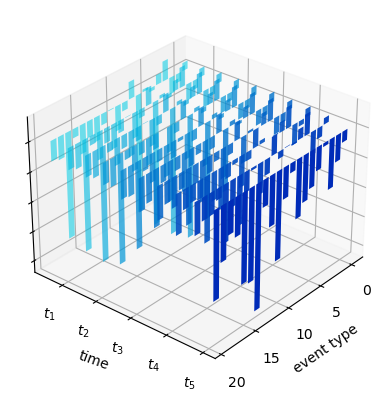
\includegraphics[width=0.92\linewidth, height = 5cm]{figure/fk_dynamic.png}
    \captionsetup[figure]{font=small, justification=justified, margin=0.1cm}
    % \vspace{-10pt}
    \captionof{figure}{Visualization of propagated $\hat{f}^*(k|t, e_i)$ in StackOverflow experiment. The each axis represent time, event type, and the magnitude. 
    The change of influence through time can be easily observed.
    }
    % \vspace{-10pt}
    \label{fig: so fk}
\end{wrapfigure} 

Our detailed investigation on the Retweet dataset further validates the explainability of Dec-ODE. 
For example, some meaningful patterns from the Retweet data is visualized in Fig. \ref{fig:retweet pattern}.
The Retweet data is composed of three classes: 
a post from a person with a small number of followers ($\sim50\%$ of the population),
a post from a person with a medium number of followers$(\sim45\%$ of the population), 
and a post from a person with a large number of followers $(\sim5\%$ of the population), denoted as 0, 1, and 2, respectively.
In Fig. \ref{fig:retweet_inten}, which visualizes $\mu(t;e_i)$ conditioned on different $e_i$, shows that each event exhibits temporally-decaying influence on $\lambda_g(t)$.
Such a pattern is expected as a post on social media shows immediate reactions, rather than a time-delayed effect.
Also, a post from an user with large followers exhibits slower decay.
Which is natural since a post from an user with a large followers gets more exposure and results in longer lasting influence on people.


\begin{figure}
    \centering
    \subfigure[Influence function $\mu(t)$ conditioned on different event types plotted on the same time range.]{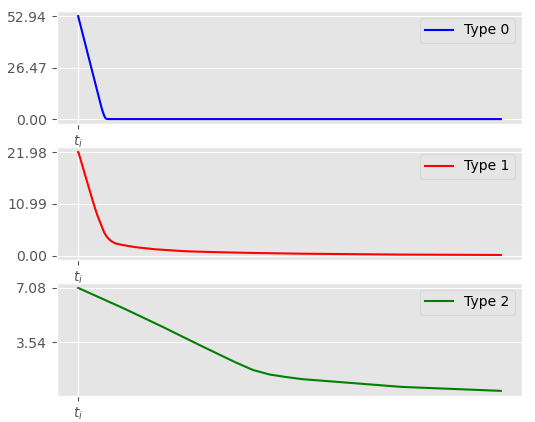
\includegraphics[width = 0.46\linewidth, height = 50mm]{figure/retweet_int.png} \label{fig:retweet_inten}} \hspace{5mm}
    \subfigure[Averaged proportion of influence from different marks on specific marks.]{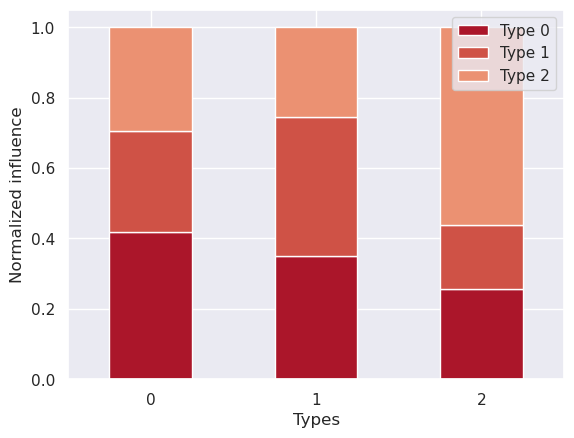
\includegraphics[width=0.46\linewidth, height = 50mm]{figure/retweet_bar.png} \label{fig:retweet_bar}}
    \subfigure[Visualization of events, i.e., marks across time, affecting each other. Blue(0): users with small followers, Red(1): users with medium followers, Green(2): users with large followers. ]{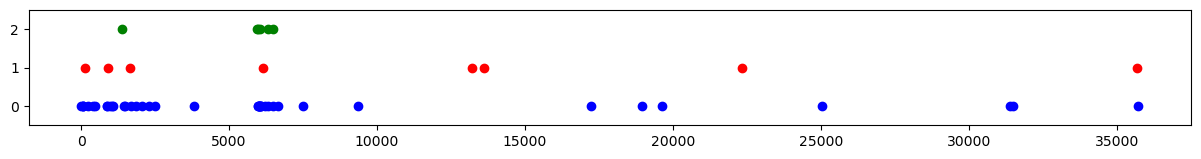
\includegraphics[width = 0.95\linewidth]{figure/retweet_dot.png}\label{fig:retweet_dot}}
    \caption{\small Visualization of patterns found in Retweet dataset. (a) $\mu(t;e_i)$ with different marks, (b) Influence of marks on each other, (c) Actual event marks with respect to time. 
    } 
    \label{fig:retweet pattern}
    % \vspace{-10pt}
\end{figure} 

Moreover, the averaged proportion of influences on different mark types are illustrated in Fig. \ref{fig:retweet_bar}.
First, even though the type 2 takes only $5\%$ of the entire population, it shows great influence in the overall occurrence of events. %This again aligns %with our %common knowledge 
This may be true as a person with many followers may have a greater influence on a broader audience. 
Second, for each event, events with the same types have the strongest influence on each other.
Considering the exponentially decaying patterns of $\mu(t)$ and the large initial magnitude of influence of type 0 shown in Fig. \ref{fig:retweet_inten}, we can infer that events with type 0 would show a high clustering effect 
and actual visualization of the data in Fig. \ref{fig:retweet_dot} validates our reasoning.


% \vspace{-5pt}
\subsection{Parallel Computing Scheme \label{ablation: parallel}}
% \vspace{-5pt}
While Neural ODEs are effective when learning the continuous dynamics of a system, the hidden state propagation requires large computation to solve IVP step by step. 
In Sec. \ref{train_parallel} we proposed to propagate the hidden state through time in parallel by disentangling individual events, 
and we validate the optimization scheme by comparing the average time for each iteration with traditional IVP. 
For the sequential propagation, a differential equation is solved from $t_0$ through $t_n$ step by step.
Table \ref{tab:parallel} summarizes the result, where the computation time significantly decreased in all cases.
Parallel computation for Dec-ODE was at least twice (for MIMIC-II) and as much as five times faster (for Reddit) than the traditional sequential computing scheme. 

\begin{table}[h]
\renewcommand{\arraystretch}{1.1}
\centering
\caption{Training efficiency comparison in different datasets with the average time taken for an iteration (sec/iter) as the metric. Ratio shows that the iteration time at least reduces in half.}
% \vspace{-8pt}
\scalebox{0.57}[0.57]{
\begin{tabular}{cc |c| cc|c | c c|c | cc|c } 
\multicolumn{3}{c|}{StackOverflow} & \multicolumn{3}{c|}{MIMIC-II} & \multicolumn{3}{c|}{Retweet} & \multicolumn{3}{c}{Reddit}\\[-2pt]
\hline
parallel &Sequential& Ratio &  parallel& Sequential&Ratio &  parallel&Sequential&Ratio &  parallel&Sequential&Ratio\\
\hline
\multirow{1}{*}{} $15.0$ & $57.7$ &0.26 & $2.9$ & $6.5$ & $0.47$ & $16.8$ & $67.6$ &$0.25$ & $15.5$ & $78.7$ & $0.20$ \\
   
\end{tabular}
}
\label{tab:parallel}
\end{table}




\section{Linear vs. Non-Linear Influence Function\label{lin-nonlin}}
In the table \ref{table: real-life}, the simple Dec-ODE with linear $\Phi_\lambda$ has been tested.
However, $\Phi_\lambda$ and $\Phi_k$ can be any functions, even neural networks, that satisfy the conditions mentioned in \ref{sec:ground int} and \ref{sec:fk}.
In fact, with linear $\Phi_\lambda$ every influence function must satisfy $\mu(t) \ge 0$ to keep the intensity positive.
Therefore, only an excitatory effect, where an event can only increase the intensity, can be expressed.

In this section, to navigate the extensibility of our framework, a less constrained variant is introduced and tested, denoted as \textit{non-linear} $\Phi_\lambda$. 
The non-linear $\Phi_\lambda(t)$ is defined as follows:
\begin{align}
    \Phi_\lambda(\mu(t;e_0), \cdots, \mu(t;e_i)) = \text{softplus} \bigg( \sum _{e_i \in \mathcal{H}_{t}}  \mu  (t; e_i) \bigg).
\end{align}
Through this modeling approach, an inhibitory effect, where an event decreases the overall intensity, can occur. 

To see how this relaxation affects in modeling TPP, both are tested in a simplified setting, where only the first 40 events of each sequence are used. The results of the experiment are summarized in Table \ref{tab:nonlin} using NLL as the metric. 
The overall result regarding the ground intensity was improved in most situations showing that the intensity function with higher fidelity can be predicted using more flexible $\Phi_\lambda$.

However, non-linear Dec-ODE shows some limitations in predicting a time-delaying effect, where an event does not have a large influence until a certain time passes rather than having an instant influence.
This happens because the inhibitory effect exceeds the excitatory effect, and the intensity function becomes $0$.
In such cases, the inhibitory effect rather impairs the model's ability.
In conclusion, this experiment suggests that with a more flexible $\Phi_\lambda$, prediction can be made with higher fidelity in most cases.
However, adding constraints has to be further discussed to robustly model different patterns in TPP.

\begin{table}[h]
\centering
\caption{Experiment on non-linear $\Phi_\lambda$. The softplus is applied after the summation in order to express inhibitory effects.}
\scalebox{0.9}[0.9]{
\begin{tabular}{cc | cc| c c | cc } \Xhline{0.3ex}
\multicolumn{2}{c|}{StackOverflow} & \multicolumn{2}{c|}{MIMIC-II} & \multicolumn{2}{c|}{Retweet} & \multicolumn{2}{c}{Reddit}\\[-2pt]
Linear & Non-linear &  Linear & Non-linear  &  Linear & Non-linear  & Linear & Non-linear\\
\hline
\multirow{1}{*}{} $0.9948$ & $\textbf{0.8987}$ &0.2451 & $\textbf{0.2183}$ & $-5.0872$ & $\textbf{-5.1649}$ & $\textbf{0.5163}$ & $18.2571$ \\
\Xhline{0.3ex}      
\end{tabular}}
    \label{tab:nonlin}
\end{table}

\section{Imputation \label{appen:imputation}}

In this section, we investigate the effect of independently modeling hidden state dynamics by comparing it with methods using contextual information.
Events from the StackOverflow dataset are randomly dropped to see how the behavior changes as the number of observed events decreases. 

\setlength{\intextsep}{0pt}
\begin{wrapfigure}{r}{0.46\textwidth}
    \centering
    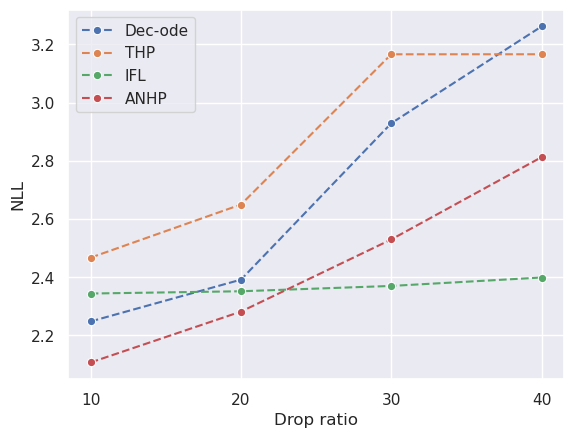
\includegraphics[width=0.44\textwidth]{figure/imputation.png}
    \caption{\raggedright Imputation experiment done using Stackoverflow dataset, where from $10\%$ to $40\%$ of data are randomly dropped.}  
    \label{fig:imputation}
\end{wrapfigure} For the fair comparison, we randomly selected 90\%, 80\%, 70\%, and 60\% indexes from the test dataset, and saved the data with the selected indexes as new test sets.
The results using the new test sets are visualized in figure \ref{fig:imputation}.
The graph illustrates that the decrease in performance of Dec-ODEs shows a similar tendency when compared to others.

The result suggests that other methods cannot retrieve the loss of information.
This statement can be made since Dec-ODE, which does not consider inter-event relationships, shows a similar tendency.

\section{Simulation Study}

\begin{table}[h]
    \centering
    \begin{tabular}{c|c|c|c}
            & RMSE   & ACC   & NLL    \\ \hline
    THP     & 0.7734 & 27.48 & 3.0121 \\ 
    ANHP    & 0.6528 & 30.31 & 0.2807 \\ 
    Dec-ODE & \textbf{0.6568} & \textbf{30.35} & \textbf{0.2739} 
    \end{tabular}
    \caption{Estimation accuracy on the simulated Hawkes process. }
        \label{tab:simulation}
    \end{table}

We have performed a simulation study on the Hawkes process following a similar procedure from the Neural Hawkes Process (NHP) \cite{bib:nhp}. 
In order to obtain the true intensity function we randomly sampled the parameters for the kernel function of the multivariate Hawkes process, and we simulated synthetic data using the tick library \cite{bacry2018tick}. 
The range of the sampling was changed from the NHP since the scale in the library was different from the paper.
In Figure \ref{fig:sim_a} - \ref{fig:sim_d}, THP struggles to simulate the flexible dynamics of the intensity function $\lambda_g$, whereas ANHP and Dec-ODE show similar dynamics to the ground truth intensity. 
The table \ref{tab:simulation} also demonstrates that Dec-ODE shows better results than THP and ANHP in all metrics. 
The result also aligns with the results in Table \ref{table: real-life}, which suggests that Dec-ODE can simulate reliable MTPPs compared to other state-of-the-art methods. 
Figure \ref{fig:sim_ae} illustrates $\mu(t)$ that compose $\lambda_g(t)$ from Figure \ref{fig:sim_d}, which shows that the ground intensity $\lambda_g(t)$ can be reconstructed from the individually constructed trajectory, i.e. an MTPP can be modeled from decoupled information.

\begin{figure}[h]
    \centering
    \subfigure[]{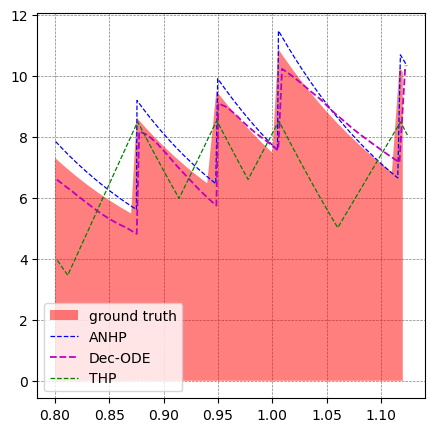
\includegraphics[height = 0.3\linewidth]{figure/total_intensity1.png}\label{fig:sim_a}}\hspace{-1mm}
    \subfigure[]{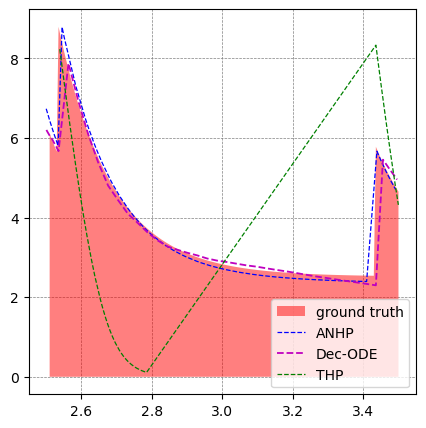
\includegraphics[height = 0.3\linewidth]{figure/total_intensity2.png}\label{fig:sim_b}}\hspace{-1mm}
    \subfigure[]{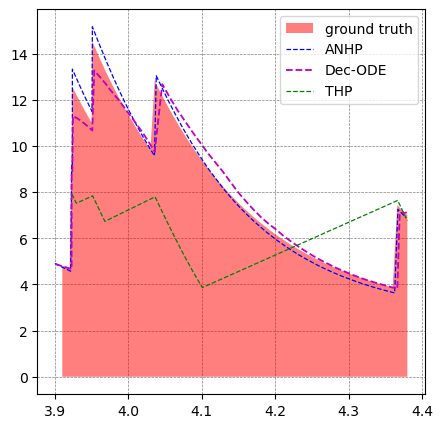
\includegraphics[height = 0.3\linewidth]{figure/total_intensity3.png}\label{fig:sim_c}}\hspace{-1mm}
    \subfigure[]{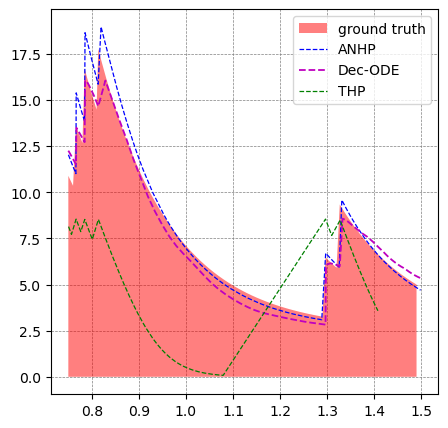
\includegraphics[height = 0.35\linewidth]{figure/total_intensity4.png}\label{fig:sim_d}}\hspace{1mm}
    \subfigure[]{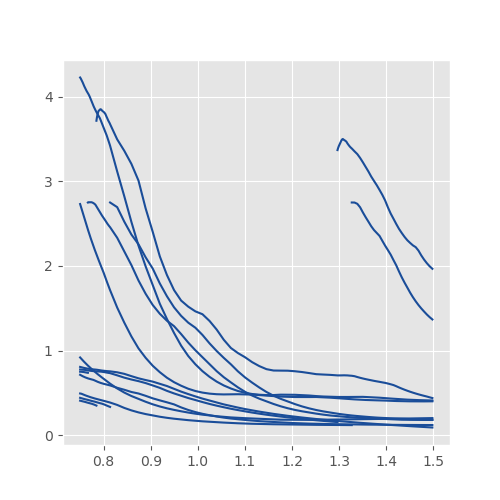
\includegraphics[height = 0.4\linewidth]{figure/decoupled_intensity4.png}\label{fig:sim_ae}}\hspace{1mm}
    \caption{Visualization from a simulation study. (a), (b), (c), and (d) compare the true intensity function of a Hawkes process and the reconstructed results from THP, ANHP, and Dec-ODEs. Each $\mu(t)$ that composes the result in (d) is illustrated in (e).}
    \label{fig:simulation}
\end{figure}



\section{Train time comparison}

In order to compare the time required for training, the time required for training one epoch (sec / epoch) is measured. The experiment is conducted on a single NVIDIA RTX A6000 GPU (48GB) with the largest batch size possible for the GPU. The result can be found in the table \ref{tab:epoch_time}. THP required the least amount of time, while methods predicting intensity at each time point showed a relatively slower training rate. In most cases, Dec-ODE shows a shorter training time per epoch.
\begin{table}[h]
    \renewcommand{\arraystretch}{1.1}
    \centering
    \caption{Training time (sec / epoch) compared between THP, ANHP, and Dec-ODE.}
    % \vspace{-8pt}
    \scalebox{0.9}[0.9]{
    \begin{tabular}{c| c| c | c | c | c } \Xhline{0.3ex}
    & \multicolumn{1}{c|}{MOOC} & \multicolumn{1}{c|}{Reddit} & \multicolumn{1}{c|}{Retweet} & \multicolumn{1}{c|}{Stackoverflow} & \multicolumn{1}{c}{MIMIC-II}\\[-2pt]
    \hline
    THP & $12.94$ & $66.95$ & $34.05$ & $13.36$ & $2.27$ \\
    ANHP & $835.36$ & $541.20$ & $630.64$ &$129.51$ & $3.69$ \\
    Dec-ODE & $117.35$ & $242.75$ & $484.08$ & $123.28$ & $8.12$\\
        
    \Xhline{0.3ex}      
    \end{tabular}
    }
        \label{tab:epoch_time}
    
    \end{table}
    
    \begin{table}[h]
    \renewcommand{\arraystretch}{1.1}
    \centering
    \caption{Required memory (MB) compared between baseline methods with batch size 4.}
    
    \scalebox{0.8}[0.8]{
    \begin{tabular}{c| c| c | c | c | c } \Xhline{0.3ex}
    & \multicolumn{1}{c|}{MOOC} & \multicolumn{1}{c|}{Reddit} & \multicolumn{1}{c|}{Retweet} & \multicolumn{1}{c|}{Stackoverflow} & \multicolumn{1}{c}{MIMIC-II}\\[-2pt]
    \hline
    RMTPP & $1110 + 1114$ & $1706 + 1142$ & $1294 + 1112$ & $1306 + 1114$ & $1114 + 1106$ \\
    THP & $3484$ & $15304$ & $1678$ & $3808$ & $1130$ \\
    ANHP & $31310$ & $< 48$ GB & $11790$ &$39260$ & $1244$ \\
    Dec-ODE & $1422$ & $1472$ & $1314$ & $1422$ & $1470$\\
    \Xhline{0.3ex}      
    \end{tabular}
    }
        \label{tab:epoch_memory}
    \end{table}
\section{Implementation details}

\subsection{IVP solving with varying time intervals \label{appen: varied time}} 
Initial Value Problem (IVP) solving with varying time intervals is done following the method introduced in \cite{bib:STPP}.
In short, the integration in the region $[t_{start}, t_{end}]$ is solved within $[0, 1]$ and scaled back to the original region. 
Using this method, every time interval with different lengths can be computed within the same number of steps.
We apply this for both batch computations with different lengths and parallel computation of $h(t;e_i)$ in Sec. \ref{train_parallel}.

\subsection{Batch Computation}
Our method propagates $h(t)$  further than $t_N$, which is the last observed point.
Therefore, in order to cover the full range of $f^*(t)$, two different masking operations are required.
The first one is the one commonly used when dealing with sequences with different lengths, and we call it the \textit{sequence mask}.
With sequences with different lengths, unobserved events should be ignored for both training and inference, and the sequence mask is used to ignore unobserved time points.
The second mask is the \textit{propagation mask}, where the unobserved time points after $t_N$ are not masked.
This is used for solving ODEs to propagate $h(t)$ until the decoded $\mu(t)$ converges.


\subsection{Baseline \label{sec:baselineImplementation}}

For THP and ANHP, we used the public GitHub \href{https://github.com/yangalan123/anhp-andtt}{repository} (\cite{bib:ANHP} with MIT License).
The code for the THP has been modified by \cite{bib:ANHP}, where time and event prediction is now made by using $\lambda(t)$ with a thinning algorithm instead of the prediction module that is parameterized by neural networks.

Moreover, as mentioned in the public GitHub repository of THP, there is an error regarding the NLL computation. In both published versions, NLL is computed conditioned on the observed history information and a current event. i.e., $L(e_i) = f(e_i|e_0, \cdots, e_i)$. Therefore, the calculation of the intensity has been corrected to $L(e_i) = f(e_i|e_0, \cdots, e_{i-1})$, where the modification is made based on the code used for the integration.

For IFL, we used the public GitHub repository \href{https://github.com/shchur/ifl-tpp}{https://github.com/shchur/ifl-tpp} (\cite{bib:ifl}, no license specified). Some modifications have been made since the original implementation does not support time point prediction. The modification was made based on the author's comment made in the ``issue'' page of the repository. However, the computation of $\mathbb{E}[t]$ was not stable due to the high variance of components in the mixture model. In other words, when a distribution in a mixture model has a high variance, the exponential term in the calculation causes an overflow, which leads to an overflow of the entire calculation. 
Therefore, we have tightened the parameters for the gradient clipping in \cite{bib:ifl}, as done in \cite{bib:MetaTPP}.


\subsection{Thinning algorithm\label{appen: thinning}}
For the experiment done in Table \ref{table: real-life}, we tested different parameters for the thinning algorithm \cite{lec:thinning, bib:thinning_ogata}, implemented by \cite{bib:ANHP}, for a fair comparison.
THP and ANHP sample the next time points using the thinning algorithm then take their average to compute $\mathbf{E}[t]$.

The thinning algorithm resembles the rejection sampling, in which the proposal is accepted with the probability $\lambda(t) / \lambda_{up}$ where $\lambda_{up} \geq \lambda(t)$ for all $t\in(t_{i-1}, \infty)$ \cite{bib:nhp}.
Therefore, reliable $\lambda_{up}$ is required to sample from the correct distribution.
If $\lambda_{up}$ is too high, all the samples would be rejected, whereas accept incorrect samples if $\lambda_{up}$ is too low.

In the implementation, $\lambda_{up}$ is calculated by $c * max(\lambda(s_0), \cdots, (s_m))$, where $c$ is a constant, $m$ is the number of samples used for the calculation, and $s_m$ is a uniformly sampled time point.
To find correct $\lambda_{up}$, for most of the reported results in Table \ref{table: real-life}, we increased the number of $m$ by $\times10$.
When overall $\lambda(t)$ is too low, the scale goes up to $1000$ in the most extreme case.

\subsection{Training Details}
When tuning the simple Dec-ODE, three different hyperparameters are considered for the model structure with the addition of an Initial Value Problem (IVP) solving method.
Three hyperparameters are the dimension of hidden state $D$, the dimension of linear layers of neural networks $N$, and the number of liner layers $L$.
We haven't fully searched for the optimal parameters for each dataset. For testing, we rather applied similar parameters to all datasets.

Throughout the experiment, $D$ was chosen from $\{32, 64\}$. However, since the dynamics of $h(t)$ is highly dependent on the information in the hidden state, we expect a higher dimension would enable the neural network to learn more difficult dynamics.

The width of linear layers $N$ is chosen between $\{128, 256\}$, and the number of layers are tested between $\{3, 4, 5\}$. In most cases, the number of layers did not show much improvement in the results.

The three hyperparameters above that showed the best result are chosen. However, in most cases, $D=64$, $N=256$, and $L=3$ were used.

In the case of IVP solver, two different methods were used training and testing. For training, Euler's method was used in most cases for efficiency. The purpose of training is to learn the dynamics of hidden state $h(t)$, and we believe Euler's method sufficiently satisfies such purpose, and we haven't thoroughly looked into the benefits of using different solvers.

During testing $\lambda_g(t)$, to make a more precise approximation, we utilize Runge-Kutta method with fixed step size, generally referred to as RK4. The computation of RK4 method is as follows:
\begin{align}
    y_{n+1} &= y_n + {h\over6}(k_1 + 2k_2 + 2k_3 + k_4)\\
    t_{n+1} &= t_n + h
\end{align}
where,
\begin{align}
k_1 &= f(t_n, y_n), \\
k_2 &= f(t_n + {h \over 2}, y_n + h {k_1 \over 2}),\\
k_3 &= f(t_n + {h \over 2}, y_n + h {k_2 \over 2}),\\
k_4 &= f(t_n + h, y_n + hk_3).
\end{align}

The RK4 method can more precisely model the trajectory compared to Euler's method. 
Therefore, there is less error in the estimated $f^*(t)$.
Other methods such as dopri5, RK4 with step size control, and other variants of IVP solvers can be applied for more accurate results.

To solve the IVP, we fixed the number of steps required for solving from $t_i$ to $t_{i+1}$. Similar to the IVP solver, we used a simpler setting for the training and a more precise setting for the testing. During training, in most cases, we used 16 steps in between every event. The increase in number is expected to improve the result, yet we have not thoroughly looked into it since it shows comparable results with state-of-the-art methods. During testing, we increased the number to 64.

When testing $f(k|t)$, the precise approximation of $\hat{f} (k|t, e_i)$ did not show a visible effect on the result.
Therefore, for computational efficiency, Euler's method was used with the same number of step sizes used for training.



\section{Dataset Description}
\begin{table}[h]
    \centering
    \renewcommand{\arraystretch}{1.3}
        \begin{tabular}{c|c c c c}
            Datasets & \# of Seq. & \# of Events & Max Seq. Length & \# of Marks \\
            \hline
             MOOC & 7,047 & 389,407 & 200 & 97 \\ 
             Reddit & 10,000 & 532,026 & 100 & 984 \\ 
             Retweet & 24,000 & 21173,533 & 264 & 3 \\ 
             StackOverflow & 6,633 & 480,414 & 736 & 22 \\ 
             MIMIC-II & 650 & 2419 & 33 & 75 \\ 
        \end{tabular}
        \caption{Statistics of benchmark datasets used for comparisons.}
        \label{tab:data_stat}
    \end{table}
% Table \ref{tab:data_stat} shows the statistics of each benchmark dataset used for testing.

\subsection{Benchmark dataset}
MIMIC-II and Retweet were from the public GitHub repository \href{https://github.com/SimiaoZuo/Transformer-Hawkes-Process} (\cite{bib:THP}, with no license specified). Others were also from the public GihtHub repository \href{https://github.com/BIRD-TAO/GNTPP} (\cite{bib:exploring_generative}, with no license specified). 

\subsection{Data preprocess}
When dealing with Mooc, Reddit, Retweet, and StackOverflow, two modifications to the dataset have been made.
First, when two events have the same time point, one of the events is removed.
We chose the latter one in the dataset.
This is because when $t_i - t_{i-1} = 0$, IFL was not able to properly estimate $f^*(t)$.
Also, in many cases, TPP assumes 2 or more events happening at the same time as improbable.
Second, as mentioned in Sec. \ref{sec:experimentSetup}, data were scaled by the standard deviation of $\{t_{i} - t_{i-1}\}_{i=0} ^n$.
When the scale of $t_i - t_{i-1}$ is too large, overflow happens during the calculations.
Therefore, we tried to make the scale similar to the results from \cite{bib:MetaTPP}, but the standard deviation was chosen since the scale was not specified in the published work.


\section{Visualizations}

From the figures, we can identify that each data show difference in dynamics. 
For instance, in $\mu(t;e_i)$ we can identify that each influence shows a delaying effect where the effect of an event affects others after some time passes.

% \subsection{Vector field}
% By employing Neural ODEs \cite{bib:node} we can visualize the overall dynamics of functions that we estimate.
% Fig. \ref{fig:vectorfields} visualizes the vector fields.
% Fig. \ref{fig:hstateVector} visualizes the first dimension of the hidden state using the StackOverflow dataset.
% The arrow represents the dynamics where the value of the tail is given as the input.
% There are some visible patterns in the dynamic forms.
% However, a certain part of the field shows very different behavior even when they receive the same input.
% It shows that the hidden state dynamics learned from the data is very complex.
% On the other hand, $\mu(t;e_i)$ visualized in Fig. \ref{fig:muVector} shows a clear tendency in the region.

% \begin{figure}[b]
%     \centering
%     \subfigure[Visualization of the hidden state dynamics with StackOverflow dataset.]{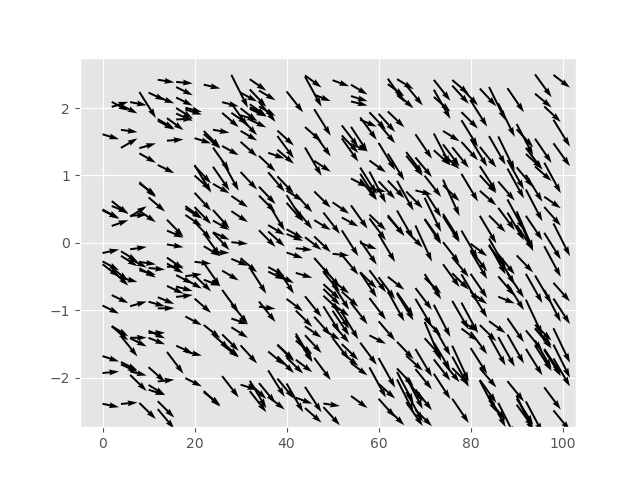
\includegraphics[width=0.45\linewidth]{figure/hs_dynamic2.png}\label{fig:hstateVector}}\hspace{5mm}
%     \subfigure[Visualization of the change of $\mu(t;e_i)$ in StackOverflow dataset. ]{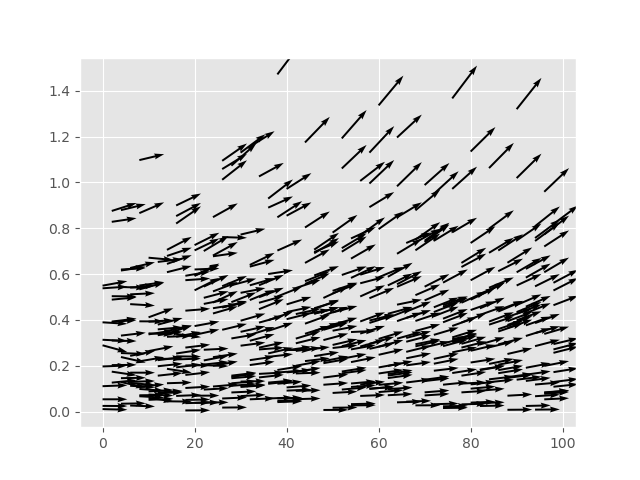
\includegraphics[width=0.45\linewidth]{figure/intensity_dynamic.png}\label{fig:muVector}}
%     \caption{Visualization of vector fields. a) is a vector field of the hidden state and b) is the vector field of $\mu(t;e_i)$. The length of the arrow represents the magnitude.}
%     \label{fig:vectorfields}
% \end{figure}
% % \vspace*{3in}

% \subsection{Visualization of Continuous Dynamics}
\begin{figure}[hb]
    % \setlength{\subfigtopskip}{0pt}   % Removes space between image and caption
    % \setlength{\subfigbottomskip}{0pt} % Removes space below the caption

    \centering
    \subfigure[Visualization of $\mu(t;e_i)$ trained using MOOC.]
    {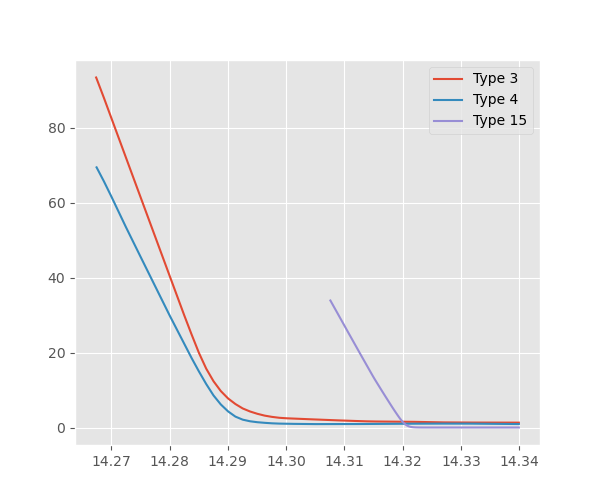
\includegraphics[height = 0.4\textwidth]{figure/mooc_inten.png}}
    \hfill
    \subfigure[\raggedright $\hat{f}(t;e_{i})$ trained using in MOOC.]
    {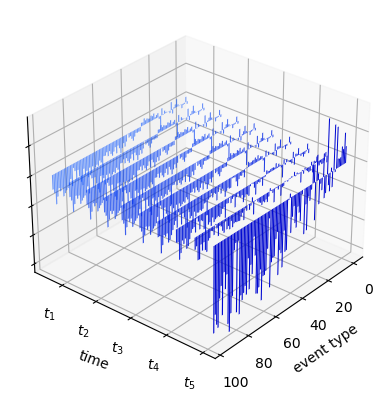
\includegraphics[height = 0.4\textwidth]
    {figure/mook_fk_14.png}}
    \caption{Visualization of dynamics of $\mu$ and $\hat{f}$ in benchmark dataset. (a) is a visualization of ground intensity trained on MOOC dataset, and (b) is a visualization of $\hat{f}(t;e_i)$ changing through time trained using MOOC dataset.}
\end{figure}

\begin{figure}[ht] \ContinuedFloat
    % \vspace{-0.3cm}
    \subfigure[$\mu(t;e_i)$ trained using Reddit.]
    {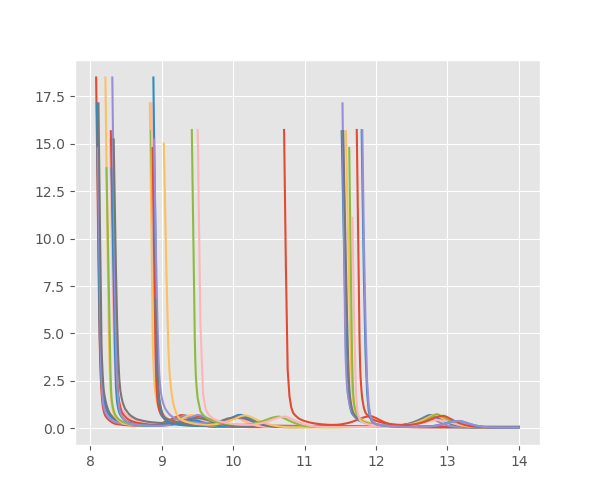
\includegraphics[height = 0.4\textwidth]{figure/reddit_inten.png}}
    \hfill
    \subfigure[\raggedright $\hat{f}(t;e_{i})$ trained on Reddit dataset.]
    {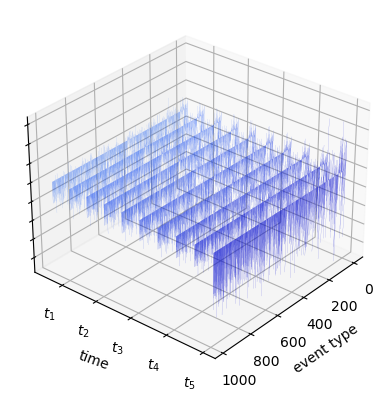
\includegraphics[height = 0.4\textwidth]
    {figure/reddit_fk_148.png}}

    % \vspace{-.3cm}
    \subfigure[Visualization of $\mu(t;e_i)$ trained using SO.]
    {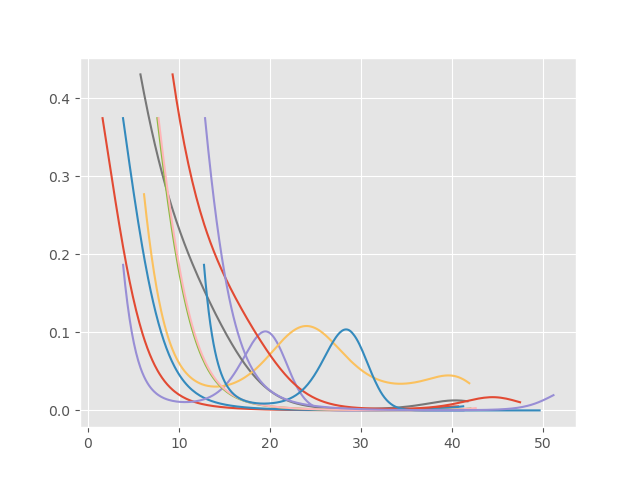
\includegraphics[height = 0.4\textwidth]{figure/SO_int.png}}
    \hfill
    \subfigure[\raggedright Visualization of $\hat{f}(t;e_{i})$ in MIMIC.]
    {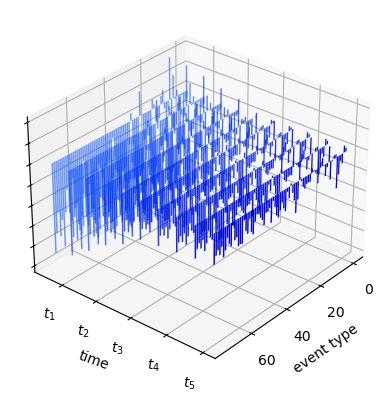
\includegraphics[height = 0.4\textwidth]{figure/mimic_fk_10.png}}
    \caption{Visualization of dynamics of $\mu$ and $\hat{f}$ in benchmark dataset. (a) is a visualization of ground intensity trained on Reddit dataset, (b) is a visualization of $\hat{f}(t;e_i)$ changing through time trained using Reddit dataset, (c) shows dynamics of ground intensity trained using Stack Overflow dataset, and (d) shows $\hat{f}(t; e_i)$ changing through time trained using MIMIC-II dataset.}
    \label{fig:mooc}

\end{figure}



\section{Comparison on Benchmarks}
This section presents a comparison between linear Dec-ODE and state-of-the-art methods using standard benchmarks.

\subsection{Experiment Setup \label{sec:experimentSetup}}
\label{sec:setup}

\textbf{Datasets.}  
We evaluated our approach on five widely-used real-world datasets from various domains:  
{\bf Reddit} represents sequences of social media posts,  
{\bf Stack Overflow (SO)} comprises sequences of rewards from the question-answering platform,  
{\bf MIMIC-II} contains sequences of diagnoses from clinical visits to the Intensive Care Unit (ICU),  
{\bf MOOC} includes sequences of user interactions with an online course,  
and {\bf Retweet} captures sequences of social media posts. Detailed descriptions of these datasets are provided in the Sec. \ref{sec:data-desc}.  
To ensure comparability across results, all time points were normalized by the standard deviation of the time gaps, $\{t_i - t_{i-1}\}_{i=1}^n$, within the training set, following the procedure outlined in \cite{bib:MetaTPP}.  

\textbf{Metrics.}  
We employed three conventional metrics for evaluation:  
1) \textit{Negative Log-Likelihood} (NLL) assesses the suitability of the predicted probability density, as computed via \eqref{eq:obj};  
2) \textit{Root Mean Squared Error} (RMSE) evaluates the accuracy of predicted event time points;  
3) \textit{Accuracy} (ACC) quantifies the correctness of the predicted mark distribution $f^*(k|t)$.  
For predictions, the expected value $\mathbb{E}_{f^*}[t]$ was used as the predicted time of the next event, and the mark with the highest probability at time $t$, i.e., $\argmax(f^*(k|t))$, was selected as the predicted mark.  

\textbf{Baseline.}  
We compared our method against four state-of-the-art approaches:  
Recurrent Marked Temporal Point Process (RMTPP) \cite{bib:RMTPP}, Transformer Hawkes Process (THP) \cite{bib:THP}, Intensity-Free Learning (IFL) \cite{bib:ifl}, and Attentive Neural Hawkes Process (ANHP) \cite{bib:ANHP}.  
Both THP and ANHP are transformer-based models that utilize the full set of observed events $\mathcal{H}_{t_n}$ to predict $e_{n+1}$.  
IFL directly models $f^*(t,k) = f^*(t) f^*(k|t)$ using a log-normal mixture for a more flexible distribution.  
As it explicitly parameterizes the distribution $f^*(t)$, the expected value $\mathbb{E}_{f^*}[t]$ can be computed analytically.  
Additional implementation details are provided in Sec.\ref{sec:baselineImplementation}.


\begin{table}[!t]
\centering
\caption{Comparison with the state of the art methods on 5 popular real-life datasets. Results with \textbf{boldface} and \underline{underline} represent the best and the second-best results, respectively. Following \cite{bib:THP, bib:ANHP} the mean and std are gained by bootstrapping 1000 times.}
\renewcommand{\arraystretch}{1.3}
\small
\scalebox{0.52}[0.52]{

\begin{tabular}{c | c c c c | c | c c c c | c | c c c c | c} 
& \multicolumn{5}{c|}{RMSE} & \multicolumn{5}{c|}{ACC} & \multicolumn{5}{c}{NLL}\\
\cline{2-6} \cline{7-11} \cline{12-16}
&  RMTPP & THP & IFL & ANHP & \textbf{Dec-ODE} & RMTPP & THP & IFL & ANHP & \textbf{Dec-ODE} & RMTPP & THP & IFL & ANHP & \textbf{Dec-ODE}\\ 
\hline
\hline
\multirow{2}{*}{MOOC} & $0.473$ & $0.476$ & $0.501$ & \underline{$0.470$} & $\textbf{0.467}$
                        & $20.98$ & $24.49$ & $\underline{32.30}$ & $31.53$ & $\textbf{42.08}$ 
                        & $-0.315$ & $0.733$ & $\textbf{-2.895}$ & $\underline{-2.632}$ & $-2.289$  \\  [-3pt]
                    & ${(0.012)}$ & $(0.010)$ & ${(0.012)}$ & $\underline{(0.019)}$ & $\textbf{(0.012)}$
                    & $(0.29)$ &${(0.22)}$ & $\underline{(1.30)}$ & $(0.20)$ & $\textbf{(0.44)}$
                    & $(0.031)$ & $(0.047)$ & $\textbf{(0.031)}$ & $(\underline{0.043})$ & ${(0.191)}$ \\[3pt]
\multirow{2}{*}{Reddit} & $\underline{0.953} $ & $6.151$ & $1.040$ & $1.149$ & $\textbf{0.934}$
                        & $29.67$ & $60.72$ & $48.91$ & $\textbf{63.45}$ & $\underline{62.32}$ 
                        & $3.559$ & $2.335$ & $2.188$ & $\textbf{1.203}$ & $\underline{1.367}$ \\[-3pt]
                        & $\underline{(0.016)}$ & $(0.195)$ &  $(0.017)$ & $(0.010)$ & $\textbf{(0.017)}$
                        & $(1.19)$ & $(0.08)$ & $(1.27)$ & $\textbf{(0.16)}$ & $\underline{(0.11)}$ 
                        & $(0.070)$ &$(0.031)$ & $(0.088)$ & $\textbf{(0.068)}$ & $\underline{(0.126)}$ \\[3pt]
\multirow{2}{*}{Retweet} & $\underline{0.990} $ & $1.055$ & $1.012$ & $1.663$ & $\textbf{0.985}$ 
                        & $51.72$ & $\textbf{60.68} $ & $55.35$ & ${59.72}$ & $\underline{60.17}$ 
                        & $-2.180$ & $-2.597$ & $-2.672$ & $\textbf{-3.134}$ & $\underline{-2.897}$ \\[-3pt]
                    & $\underline{(0.016)}$ & $(0.015)$ & $(0.018)$ & $(0.014)$ & $\textbf{(0.016)}$
                    & $(0.33)$ & $\textbf{(0.11)}$ & $(0.19)$ & $(0.11)$ & $\underline{(0.23)}$ 
                    & $(0.025)$ & $(0.016)$ & $(0.023)$ & $\textbf{(0.019)}$ & $\underline{(0.030)}$ \\[3pt]
\multirow{2}{*}{MIMIC-II} & $\underline{0.859} $ & $>10$ & $1.005$ & $0.933$ & $\textbf{0.810}$ 
                        & $78.20$ & $\textbf{85.98} $ & $80.49$ & $84.30$ & $\underline{85.06}$ 
                        & $1.167$ & $5.657$ & $\textbf{0.939} $ & $\underline{1.025}$ & $1.354$ \\  [-3pt]
                    & $\underline{(0.093)} $ & $(0.114)$ & $(0.121)$ & $(0.088)$ & $\textbf{(0.173)}$
                    & $(5.00)$ & $\textbf{(2.56)} $ & $(5.20)$ & $(2.78)$ & $\underline{(3.65)}$ 
                    & $(0.150)$ & $(0.304)$ & $\textbf{(0.139)} $ & $\underline{(0.155)}$ & $(0.413)$ \\[3pt]
\multirow{2}{*}{} \text{Stack} & $\textbf{1.017} $ & $1.057$ & $1.340$ & $1.052$ & $\underline{1.018}$
                    & $53.95$ & $53.83$ & $53.00$ & $\textbf{56.80}$ & $\underline{55.58}$ 
                    & $2.156$ &$2.318$ & $2.314$ & $\textbf{1.873}$ & $\underline{2.063}$  \\ [-3pt]
                    \text{Overflow} &  $\textbf{(0.011)}$ & $(0.011)$ & $(0.013)$ & $(0.011)$ & $\underline{(0.011)}$
                    & $(0.32)$ & $(0.18)$ & $(0.35)$ & $\textbf{(0.18)} $ & $\underline{(0.29)}$ 
                    & $(0.022)$ & $(0.022)$ & $(0.020)$ & $\textbf{(0.017)} $ & $\underline{(0.016)}$     \\[3pt]
                    \hline
\end{tabular}}
\label{table: real-life}
\end{table}

\subsection{Comparison of Results}
\label{sec: real-life}

We evaluate the performance of linear Dec-ODE against state-of-the-art TPP methods using the five real-world datasets described in Sec. \ref{sec:setup}. A summary of the results is provided in Table \ref{table: real-life}.  
Overall, our approach achieved results that were comparable to or better than the baselines across all metrics.  
This demonstrates that Dec-ODE effectively captures the complex dynamics of MTPPs through independently propagated influence functions.  
Notably, Dec-ODE excelled in prediction tasks, as evidenced by its low RMSE, while ANHP slightly outperformed it in NLL. Additionally, methods like Dec-ODE and IFL, which estimate $f^*(t)$ to compute $\mathbb{E}[t]$, tended to predict event times more accurately.  

\textbf{Discussion.}  
To ensure a fair comparison, we increased the number of samples used in the thinning algorithm \cite{lec:thinning, bib:thinning_ogata} implemented by \cite{bib:ANHP}. In most cases, the sample count was increased by a factor of 20. However, on the Reddit dataset with THP, the thinning algorithm struggled to sample correctly from $f^*(t)$ due to the low magnitude and high fluctuation of the intensity function. Additional details are provided in Sec.\ref{appen: thinning}.

\subsection{Explainability of Dec-ODE\label{exp: explainability}}

In MTPP and TPP, events have a temporal and complex influence on $\lambda^*(t)$ and $f^*(t)$ \cite{bib:hawkesOrigin, ISHAM1979335}.  
Thus, when evaluating the explainability of a neural network modeling an MTPP, it is crucial to understand how individual events impact predictions and how these effects evolve over time.  
Dec-ODE inherently provides this information.  
For instance, the temporal behavior of $\lambda_g^*(t)$ and $\hat{f}^*(k|t)$ can be directly visualized, as shown in Fig. \ref{fig: so fk}.

\begin{wrapfigure}{r}{0.40\textwidth}
    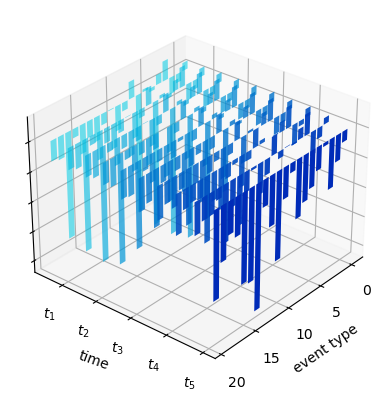
\includegraphics[width=0.92\linewidth, height=5cm]{figure/fk_dynamic.png}
    \captionsetup[figure]{font=small, justification=justified, margin=0.1cm}
    \captionof{figure}{Visualization of propagated $\hat{f}^*(k|t, e_i)$ in the StackOverflow experiment. The axes represent time, event type, and magnitude, respectively.}
    \label{fig: so fk}
\end{wrapfigure}

Our detailed analysis of the Retweet dataset further corroborates Dec-ODE's explainability.  
For example, meaningful patterns in the Retweet data are visualized in Fig. \ref{fig:retweet pattern}.  
The dataset comprises three classes:  
a post by a user with few followers ($\sim50\%$ of the population),  
a post by a user with a moderate number of followers ($\sim45\%$),  
and a post by a user with many followers ($\sim5\%$), labeled as 0, 1, and 2, respectively.  
In Fig. \ref{fig:retweet_inten}, which visualizes $\mu(t; e_i)$ conditioned on different $e_i$, each event shows a temporally decaying influence on $\lambda_g(t)$.  
This aligns with the expected behavior of social media posts, which generally elicit immediate reactions rather than delayed effects. 
Moreover, posts from users with many followers exhibit slower decay, as they tend to have broader exposure and sustain their influence for a longer time.

\begin{figure}
    \centering
    \subfigure[Influence function $\mu(t)$ conditioned on different event types, plotted over the same time range.]{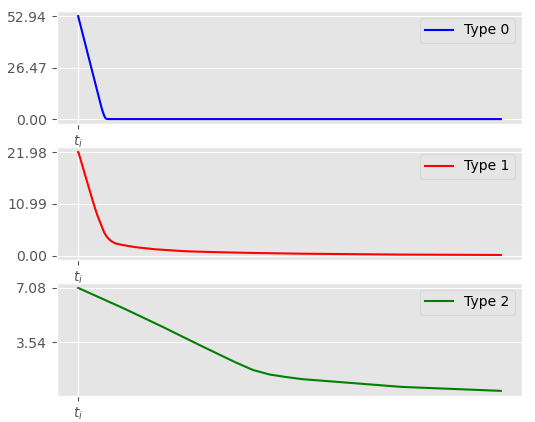
\includegraphics[width=0.46\linewidth, height=50mm]{figure/retweet_int.png} \label{fig:retweet_inten}} \hspace{5mm}
    \subfigure[Averaged influence proportions between different marks.]{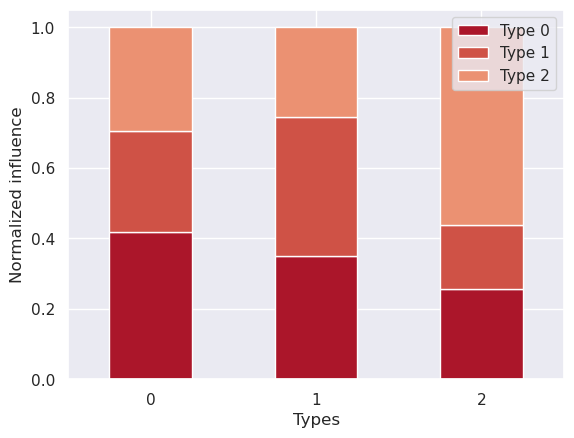
\includegraphics[width=0.46\linewidth, height=50mm]{figure/retweet_bar.png} \label{fig:retweet_bar}}
    \subfigure[Visualization of event marks over time. Blue (0): users with few followers, Red (1): users with moderate followers, Green (2): users with many followers.]{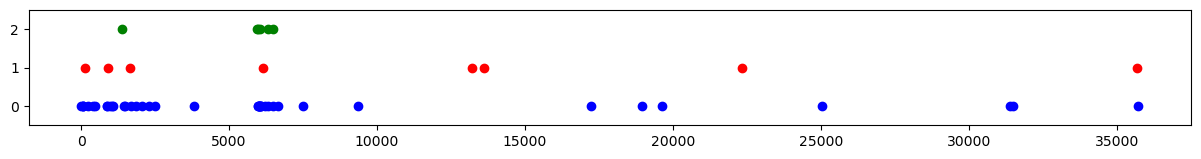
\includegraphics[width=0.95\linewidth]{figure/retweet_dot.png} \label{fig:retweet_dot}}
    \caption{\small Visualization of patterns in the Retweet dataset. (a) $\mu(t; e_i)$ for different marks, (b) Interaction between marks, (c) Event marks over time.}
    \label{fig:retweet pattern}
\end{figure}

Furthermore, the averaged proportions of influence across different mark types are shown in Fig. \ref{fig:retweet_bar}.  
First, despite type 2 accounting for only $5\%$ of the population, it exerts significant influence on the overall occurrence of events.  
This is consistent with the notion that individuals with many followers tend to impact a larger audience.  
Second, events of the same type have the strongest mutual influence.  
Given the exponentially decaying pattern of $\mu(t)$ and the large initial influence magnitude of type 0 (Fig. \ref{fig:retweet_inten}), events of type 0 likely exhibit strong clustering.  
This inference is validated by the visualization in Fig. \ref{fig:retweet_dot}.



\subsection{Parallel Computing Scheme \label{ablation: parallel}}
While Neural ODEs are highly effective at learning the continuous dynamics of a system, propagating the hidden state requires solving the IVP step by step, which can be computationally intensive.  
In Sec. \ref{train_parallel}, we introduced a method to propagate the hidden state through time in parallel by disentangling individual events.  
We validate this optimization scheme by comparing the average iteration time with that of traditional IVP-based sequential propagation.  

For the sequential approach, the differential equation is solved incrementally from $t_0$ to $t_n$.  
Table \ref{tab:parallel} presents the results, demonstrating a significant reduction in computation time across all cases.  
The parallelized computation for Dec-ODE was at least twice as fast (e.g., for MIMIC-II) and up to five times faster (e.g., for Reddit) compared to the traditional sequential scheme.

\begin{table}[h]
\renewcommand{\arraystretch}{1.1}
\centering
\caption{Training efficiency comparison in different datasets with the average time taken for an iteration (sec/iter) as the metric. Ratio shows that the iteration time at least reduces in half.}
\scalebox{0.6}[0.6]{
\begin{tabular}{cc |c| cc|c | c c|c | cc|c } 
\multicolumn{3}{c|}{StackOverflow} & \multicolumn{3}{c|}{MIMIC-II} & \multicolumn{3}{c|}{Retweet} & \multicolumn{3}{c}{Reddit}\\[-2pt]
\hline
parallel &Sequential& Ratio &  parallel& Sequential&Ratio &  parallel&Sequential&Ratio &  parallel&Sequential&Ratio\\
\hline
\multirow{1}{*}{} $15.0$ & $57.7$ &0.26 & $2.9$ & $6.5$ & $0.47$ & $16.8$ & $67.6$ &$0.25$ & $15.5$ & $78.7$ & $0.20$ \\
   
\end{tabular}
}
\label{tab:parallel}
\end{table}


\section{Linear vs. Non-Linear Influence Function\label{lin-nonlin}}  
In Table \ref{table: real-life}, the basic Dec-ODE model with a linear $\Phi_\lambda$ was evaluated.  
However, both $\Phi_\lambda$ and $\Phi_k$ can be defined as any functions, including neural networks, as long as they meet the conditions outlined in Secs. \ref{sec:ground int} and \ref{sec:fk}.  
Notably, with a linear $\Phi_\lambda$, every influence function must satisfy $\mu(t) \ge 0$ to ensure the intensity remains positive.  
This constraint means that only excitatory effects, where events increase the intensity, can be modeled.  

In this section, we explore the extensibility of our framework by introducing and testing a less restricted variant, referred to as the \textit{non-linear} $\Phi_\lambda$.  
The non-linear $\Phi_\lambda(t)$ is defined as follows:

\begin{align}
    \Phi_\lambda(\mu(t;e_0), \cdots, \mu(t;e_i)) = \text{softplus} \bigg( \sum _{e_i \in \mathcal{H}_{t}}  \mu  (t; e_i) \bigg).
\end{align}

Through this modeling approach, inhibitory effects, where an event reduces the overall intensity, can be incorporated.

To assess how this relaxation influences the modeling of TPP, both linear and non-linear models are tested in a simplified setting, using only the first 40 events from each sequence. The experimental results are summarized in Table \ref{tab:nonlin}, with NLL as the evaluation metric.  
In most cases, the overall result regarding the ground intensity improved, indicating that a more flexible $\Phi_\lambda$ allows for a more accurate prediction of the intensity function.

However, the non-linear Dec-ODE model reveals limitations when predicting time-delayed effects, where an event does not immediately influence the intensity but instead has a delayed effect. This issue arises because the inhibitory effect outweighs the excitatory one, causing the intensity function to drop to zero. In such situations, the inhibitory effect hinders the model's performance.

In conclusion, this experiment suggests that a more flexible $\Phi_\lambda$ can lead to higher fidelity predictions in most cases. However, further discussion is needed regarding the introduction of constraints to more effectively model various patterns in TPP.


\begin{table}[h]
\centering
\caption{Experiment on non-linear $\Phi_\lambda$. The softplus is applied after the summation in order to express inhibitory effects.}
\scalebox{0.9}[0.9]{
\begin{tabular}{cc | cc| c c | cc } \Xhline{0.3ex}
\multicolumn{2}{c|}{StackOverflow} & \multicolumn{2}{c|}{MIMIC-II} & \multicolumn{2}{c|}{Retweet} & \multicolumn{2}{c}{Reddit}\\[-2pt]
Linear & Non-linear &  Linear & Non-linear  &  Linear & Non-linear  & Linear & Non-linear\\
\hline
\multirow{1}{*}{} $0.9948$ & $\textbf{0.8987}$ &0.2451 & $\textbf{0.2183}$ & $-5.0872$ & $\textbf{-5.1649}$ & $\textbf{0.5163}$ & $18.2571$ \\
\Xhline{0.3ex}      
\end{tabular}}
    \label{tab:nonlin}
\end{table}

\section{Imputation \label{appen:imputation}}
In this section, we explore the impact of independently modeling hidden state dynamics by comparing it with methods that utilize contextual information. 
To examine this, events from the StackOverflow dataset are randomly removed to observe how the behavior changes as the number of observed events decreases.

\setlength{\intextsep}{0pt}
\begin{wrapfigure}{r}{0.46\textwidth}
    \centering
    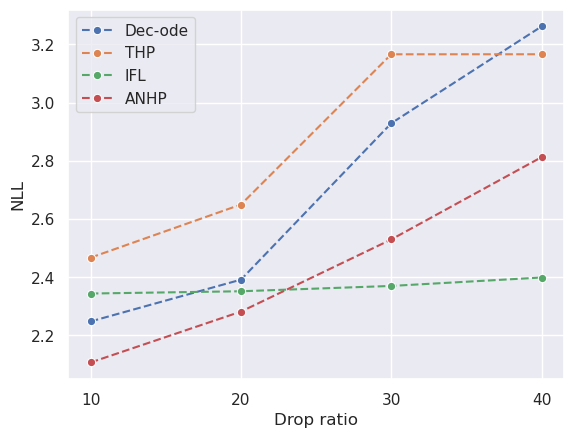
\includegraphics[width=0.44\textwidth]{figure/imputation.png}
    \caption{\raggedright Imputation experiment done using Stackoverflow dataset, where from $10\%$ to $40\%$ of data are randomly dropped.}  
    \label{fig:imputation}
\end{wrapfigure} 

For a fair comparison, we randomly selected 90\%, 80\%, 70\%, and 60\% of the indexes from the test dataset, and saved the corresponding data as new test sets. 
The results using these new test sets are visualized in Figure \ref{fig:imputation}.
The graph shows that the performance decline of Dec-ODE follows a similar trend when compared to other methods.

This suggests that the other methods are unable to recover from the loss of information. 
This conclusion is supported by the fact that Dec-ODE, which does not account for inter-event relationships, exhibits a similar trend.

\clearpage
\section{Simulation Study}


    \begin{figure}[!h]
        \centering
        \subfigure[]{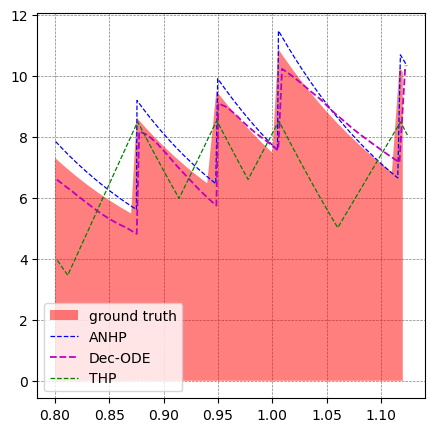
\includegraphics[height = 0.3\linewidth]{figure/total_intensity1.png}\label{fig:sim_a}}\hspace{-1mm}
        \subfigure[]{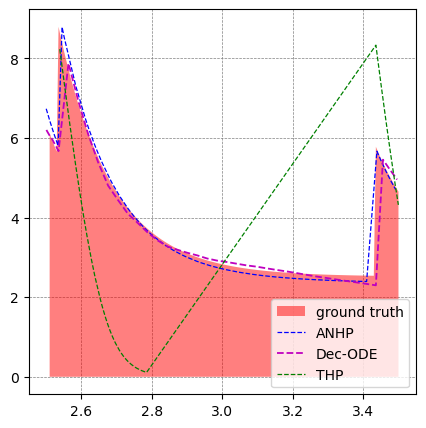
\includegraphics[height = 0.3\linewidth]{figure/total_intensity2.png}\label{fig:sim_b}}\hspace{-1mm}
        \subfigure[]{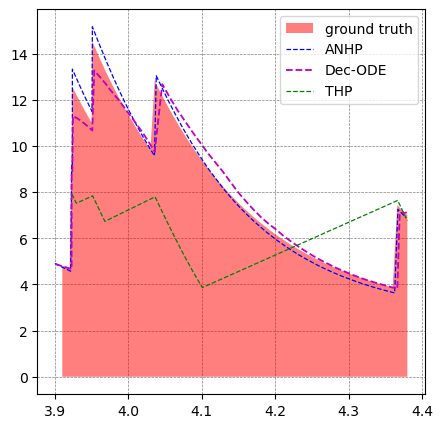
\includegraphics[height = 0.3\linewidth]{figure/total_intensity3.png}\label{fig:sim_c}}\hspace{-1mm}
        \subfigure[]{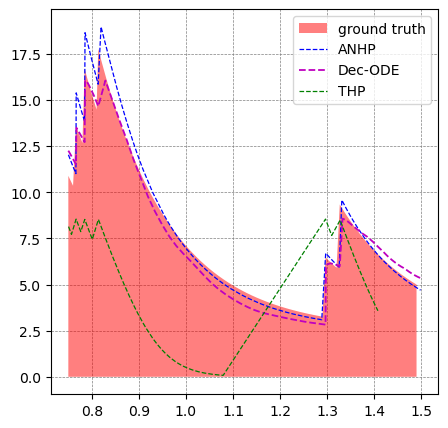
\includegraphics[height = 0.35\linewidth]{figure/total_intensity4.png}\label{fig:sim_d}}\hspace{1mm}
        \subfigure[]{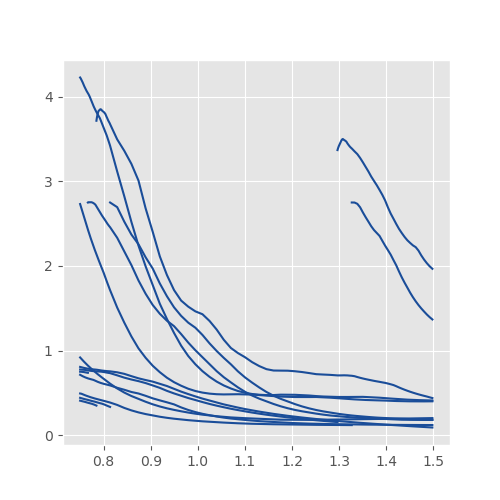
\includegraphics[height = 0.4\linewidth]{figure/decoupled_intensity4.png}\label{fig:sim_ae}}\hspace{1mm}
        \caption{Visualization from a simulation study. (a), (b), (c), and (d) compare the true intensity function of a Hawkes process and the reconstructed results from THP, ANHP, and Dec-ODEs. Each $\mu(t)$ that composes the result in (d) is illustrated in (e).}
        \label{fig:simulation}
    \end{figure}
    
    \begin{table}[h]
        \centering
        \begin{tabular}{c|c|c|c}
                & RMSE   & ACC   & NLL    \\ \hline
        THP     & 0.7734 & 27.48 & 3.0121 \\ 
        ANHP    & 0.6528 & 30.31 & 0.2807 \\ 
        Dec-ODE & \textbf{0.6568} & \textbf{30.35} & \textbf{0.2739} 
        \end{tabular}
        \caption{Estimation accuracy on the simulated Hawkes process. }
            \label{tab:simulation}
        \end{table}

We conducted a simulation study on the Hawkes process, following a similar procedure to that of the Neural Hawkes Process (NHP) \cite{bib:nhp}. 
To obtain the true intensity function, we randomly sampled parameters for the kernel function of the multivariate Hawkes process and simulated synthetic data using the tick library \cite{bacry2018tick}. 
The sampling range was adjusted from the NHP due to differences in scale between the library and the original paper.
In Figures \ref{fig:sim_a} - \ref{fig:sim_d}, THP struggles to capture the flexible dynamics of the intensity function $\lambda_g$, while ANHP and Dec-ODE exhibit dynamics closely resembling the ground truth intensity. 
Table \ref{tab:simulation} further shows that Dec-ODE outperforms both THP and ANHP across all metrics. 
These results align with those in Table \ref{table: real-life}, suggesting that Dec-ODE is capable of reliably simulating MTPPs compared to other state-of-the-art methods. 
Figure \ref{fig:sim_ae} visualizes $\mu(t)$ components that make up $\lambda_g(t)$ from Figure \ref{fig:sim_d}, demonstrating that the ground intensity $\lambda_g(t)$ can be reconstructed from the individually modeled trajectories, i.e., an MTPP can be effectively modeled using decoupled information.


\section{Train time comparison}

The time required for training one epoch (sec / epoch) is measured in order to compare the time required for training. 
The experiment is conducted using a single NVIDIA RTX A6000 GPU (48GB memory) with the largest batch size possible. 
The summary of the expriment can be found in the table \ref{tab:epoch_time}. 
THP required the least amount of time, while methods predicting continuous dynamics of intensity showed a relatively slower training rate. 
In most cases, Dec-ODE shows a shorter training time per epoch.
\begin{table}[h]
    \renewcommand{\arraystretch}{1.1}
    \centering
    \caption{Training time (sec / epoch) compared between THP, ANHP, and Dec-ODE.}
    % \vspace{-8pt}
    \scalebox{0.9}[0.9]{
    \begin{tabular}{c| c| c | c | c | c } \Xhline{0.3ex}
    & \multicolumn{1}{c|}{MOOC} & \multicolumn{1}{c|}{Reddit} & \multicolumn{1}{c|}{Retweet} & \multicolumn{1}{c|}{Stackoverflow} & \multicolumn{1}{c}{MIMIC-II}\\[-2pt]
    \hline
    THP & $12.94$ & $66.95$ & $34.05$ & $13.36$ & $2.27$ \\
    ANHP & $835.36$ & $541.20$ & $630.64$ &$129.51$ & $3.69$ \\
    Dec-ODE & $117.35$ & $242.75$ & $484.08$ & $123.28$ & $8.12$\\
        
    \Xhline{0.3ex}      
    \end{tabular}
    }
        \label{tab:epoch_time}
    
    \end{table}
    
    \begin{table}[h]
    \renewcommand{\arraystretch}{1.1}
    \centering
    \caption{Required memory (MB) compared between baseline methods with batch size 4.}
    
    \scalebox{0.8}[0.8]{
    \begin{tabular}{c| c| c | c | c | c } \Xhline{0.3ex}
    & \multicolumn{1}{c|}{MOOC} & \multicolumn{1}{c|}{Reddit} & \multicolumn{1}{c|}{Retweet} & \multicolumn{1}{c|}{Stackoverflow} & \multicolumn{1}{c}{MIMIC-II}\\[-2pt]
    \hline
    RMTPP & $1110 + 1114$ & $1706 + 1142$ & $1294 + 1112$ & $1306 + 1114$ & $1114 + 1106$ \\
    THP & $3484$ & $15304$ & $1678$ & $3808$ & $1130$ \\
    ANHP & $31310$ & $< 48$ GB & $11790$ &$39260$ & $1244$ \\
    Dec-ODE & $1422$ & $1472$ & $1314$ & $1422$ & $1470$\\
    \Xhline{0.3ex}      
    \end{tabular}
    }
        \label{tab:epoch_memory}
    \end{table}
\section{Implementation details}

\subsection{IVP solving with varying time intervals \label{appen: varied time}} 
The Initial Value Problem (IVP) solving with varying time intervals is performed following the approach outlined in \cite{bib:STPP}. 
In brief, the integration over the region $[t_{start}, t_{end}]$ is solved within the normalized interval $[0, 1]$, and then rescaled back to the original time range. 
This method allows for the computation of time intervals of different lengths with the same number of steps. 
We apply this technique to both batch computations with varying lengths and the parallel computation of $h(t;e_i)$ as discussed in Sec. \ref{train_parallel}.

\subsection{Batch Computation}
Our method extends the propagation of $h(t)$ beyond $t_N$, the last observed time point. 
To fully cover the range of $f^*(t)$, two distinct masking operations are necessary. 
The first is the commonly used \textit{sequence mask}, which is applied when dealing with sequences of varying lengths. 
For sequences with different lengths, unobserved events must be ignored during both training and inference, and the sequence mask serves to mask out these unobserved time points. 
The second mask is the \textit{propagation mask}, which ensures that the unobserved time points after $t_N$ are not masked. 
This mask is used when solving ODEs to propagate $h(t)$ until the decoded $\mu(t)$ reaches convergence.


\subsection{Baseline \label{sec:baselineImplementation}}

For THP and ANHP, we utilized the public GitHub \href{https://github.com/yangalan123/anhp-andtt}{repository} (\cite{bib:ANHP} with MIT License). 
The code for THP has been modified by \cite{bib:ANHP}, where time and event prediction is now performed using $\lambda(t)$ with a thinning algorithm, as opposed to the neural network-based prediction module from the original version.

Additionally, as noted in the public GitHub repository of THP, there is an issue with the NLL computation. In both published versions, NLL is computed conditioned on the observed history and the current event, i.e., $L(e_i) = f(e_i|e_0, \dots, e_i)$. Therefore, the intensity calculation has been corrected to $L(e_i) = f(e_i|e_0, \dots, e_{i-1})$, based on the integration code modifications.

For IFL, we used the public GitHub repository \href{https://github.com/shchur/ifl-tpp}{https://github.com/shchur/ifl-tpp} (\cite{bib:ifl}, no license specified). Several modifications were necessary, as the original implementation does not support time point prediction. These changes were based on the author's comments in the repository's ``issue" page. However, the computation of $\mathbb{E}[t]$ was unstable due to the high variance in the mixture model components. Specifically, when a distribution in the mixture model has high variance, the exponential term in the calculation causes an overflow, leading to an overall failure of the computation. To address this, we tightened the gradient clipping parameters in \cite{bib:ifl}, as recommended in \cite{bib:MetaTPP}.


\subsection{Thinning algorithm\label{appen: thinning}}
In the experiment presented in Table \ref{table: real-life}, we tested various parameters for the thinning algorithm \cite{lec:thinning, bib:thinning_ogata}, as implemented by \cite{bib:ANHP}, to ensure a fair comparison. 
THP and ANHP use the thinning algorithm to sample the next time points and then compute $\mathbf{E}[t]$ by averaging these samples.

The thinning algorithm operates similarly to rejection sampling, where a proposal is accepted with the probability $\lambda(t) / \lambda_{up}$, with the condition that $\lambda_{up} \geq \lambda(t)$ for all $t \in (t_{i-1}, \infty)$ \cite{bib:nhp}. 
Thus, a reliable value for $\lambda_{up}$ is crucial to sample from the correct distribution. 
If $\lambda_{up}$ is set too high, all samples will be rejected, whereas if it is set too low, incorrect samples will be accepted.

In the implementation, $\lambda_{up}$ is calculated as $c \times \max(\lambda(s_0), \dots, \lambda(s_m))$, where $c$ is a constant, $m$ is the number of samples used for the calculation, and $s_m$ is a uniformly sampled time point. 
To obtain an accurate $\lambda_{up}$, for most of the reported results in Table \ref{table: real-life}, we increased $m$ by a factor of 10. 
In cases where the overall $\lambda(t)$ is very low, the scale of $\lambda_{up}$ was increased up to 1000 in extreme cases.


\subsection{Training Details}
When tuning the simple Dec-ODE, three hyperparameters were considered for the model structure, alongside the Initial Value Problem (IVP) solving method. The hyperparameters are the dimension of the hidden state $D$, the dimension of the linear layers of the neural network $N$, and the number of linear layers $L$. We did not conduct an exhaustive search for the optimal parameters for each dataset; instead, we applied similar parameters across all datasets for testing.

Throughout the experiment, $D$ was selected from $\{32, 64\}$. Since the dynamics of $h(t)$ heavily depend on the information in the hidden state, we anticipate that a higher dimension allows the neural network to capture more complex dynamics.

The width of the linear layers $N$ was chosen from $\{128, 256\}$, and the number of layers $L$ was tested from $\{3, 4, 5\}$. In most cases, varying the number of layers did not yield significant improvements in performance.

The best-performing hyperparameters were selected based on the results, with $D=64$, $N=256$, and $L=3$ being used most frequently.

For the IVP solver, two different methods were used for training and testing. During training, Euler's method was primarily used for efficiency. Since the goal of training is to learn the dynamics of the hidden state $h(t)$, we believe that Euler's method sufficiently meets this purpose, though we did not extensively explore the benefits of other solvers.

For testing $\lambda_g(t)$, we used the more accurate Runge-Kutta method with a fixed step size, commonly referred to as RK4. The RK4 method computes the solution as follows:
\begin{align}
    y_{n+1} &= y_n + \frac{h}{6}(k_1 + 2k_2 + 2k_3 + k_4) \\
    t_{n+1} &= t_n + h
\end{align}
where,
\begin{align}
k_1 &= f(t_n, y_n), \\
k_2 &= f(t_n + \frac{h}{2}, y_n + \frac{h}{2} k_1), \\
k_3 &= f(t_n + \frac{h}{2}, y_n + \frac{h}{2} k_2), \\
k_4 &= f(t_n + h, y_n + h k_3).
\end{align}

The RK4 method provides a more precise trajectory than Euler's method, reducing the error in the estimated $f^*(t)$. Other methods, such as dopri5, RK4 with step-size control, and other IVP solver variants, can be applied for even more accurate results. However, applicaiton of such methods were not fully explored in this study.

For solving the IVP, we fixed the number of steps required to solve the interval from $t_i$ to $t_{i+1}$. Similar to the IVP solver, a simpler setting was used for training and a more precise setting for testing. During training, 16 steps were used between each event. Although increasing the number of steps is expected to improve results, we did not explore this in detail since it produced comparable results to state-of-the-art methods. For testing, the number of steps was increased to 64.

When testing $f(k|t)$, the precise approximation of $\hat{f}(k|t, e_i)$ had no noticeable effect on the results. Therefore, for computational efficiency, Euler's method was used with the same number of steps as used during training.


\section{Dataset Description \label{sec:data-desc}}
\begin{table}[h]
    \centering
    \renewcommand{\arraystretch}{1.3}
        \begin{tabular}{c|c c c c}
            Datasets & \# of Seq. & \# of Events & Max Seq. Length & \# of Marks \\
            \hline
             MOOC & 7,047 & 389,407 & 200 & 97 \\ 
             Reddit & 10,000 & 532,026 & 100 & 984 \\ 
             Retweet & 24,000 & 21173,533 & 264 & 3 \\ 
             StackOverflow & 6,633 & 480,414 & 736 & 22 \\ 
             MIMIC-II & 650 & 2419 & 33 & 75 \\ 
        \end{tabular}
        \caption{Statistics of benchmark datasets used for comparisons.}
        \label{tab:data_stat}
    \end{table}
% Table \ref{tab:data_stat} shows the statistics of each benchmark dataset used for testing.

\subsection{Benchmark dataset}
MIMIC-II and Retweet were from the public GitHub repository \href{https://github.com/SimiaoZuo/Transformer-Hawkes-Process} (\cite{bib:THP}, with no license specified). Others were also from the public GihtHub repository \href{https://github.com/BIRD-TAO/GNTPP} (\cite{bib:exploring_generative}, with no license specified). 

\subsection{Data preprocess}
When working with the Mooc, Reddit, Retweet, and StackOverflow datasets, two modifications were made. First, when two events have the same time point, one of them is removed, specifically the latter event in the dataset. This adjustment was made because when $t_i - t_{i-1} = 0$, the IFL method was unable to properly estimate $f^*(t)$. Additionally, in many cases, TPP assumes that two or more events occurring at the same time is highly improbable.

Second, as mentioned in Sec. \ref{sec:experimentSetup}, the data were scaled by the standard deviation of $\{t_{i} - t_{i-1}\}_{i=0}^n$. When the scale of $t_i - t_{i-1}$ is excessively large, it can cause overflow during computations. To mitigate this, we aimed to match the scale to the results from \cite{bib:MetaTPP}, although the exact scaling factor was not specified in the original work, so we chose the standard deviation as the scaling method.


\section{Visualizations}

% From the figures, we can identify that each data show difference in dynamics. 
% For instance, in $\mu(t;e_i)$ we can identify that each influence shows a delaying effect where the effect of an event affects others after some time passes.

% \subsection{Vector field}
% By employing Neural ODEs \cite{bib:node} we can visualize the overall dynamics of functions that we estimate.
% Fig. \ref{fig:vectorfields} visualizes the vector fields.
% Fig. \ref{fig:hstateVector} visualizes the first dimension of the hidden state using the StackOverflow dataset.
% The arrow represents the dynamics where the value of the tail is given as the input.
% There are some visible patterns in the dynamic forms.
% However, a certain part of the field shows very different behavior even when they receive the same input.
% It shows that the hidden state dynamics learned from the data is very complex.
% On the other hand, $\mu(t;e_i)$ visualized in Fig. \ref{fig:muVector} shows a clear tendency in the region.

% \begin{figure}[b]
%     \centering
%     \subfigure[Visualization of the hidden state dynamics with StackOverflow dataset.]{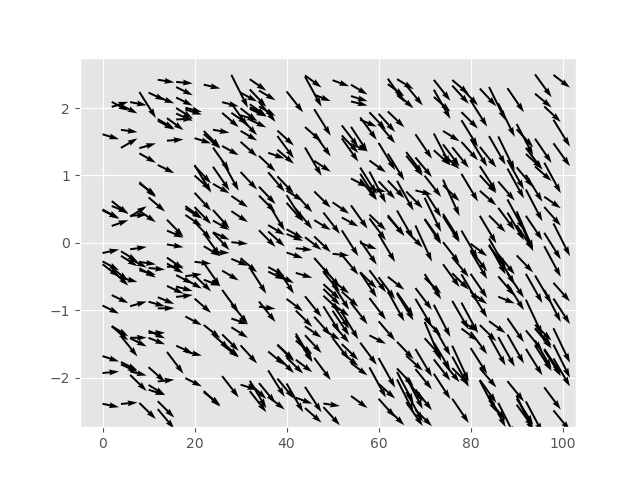
\includegraphics[width=0.45\linewidth]{figure/hs_dynamic2.png}\label{fig:hstateVector}}\hspace{5mm}
%     \subfigure[Visualization of the change of $\mu(t;e_i)$ in StackOverflow dataset. ]{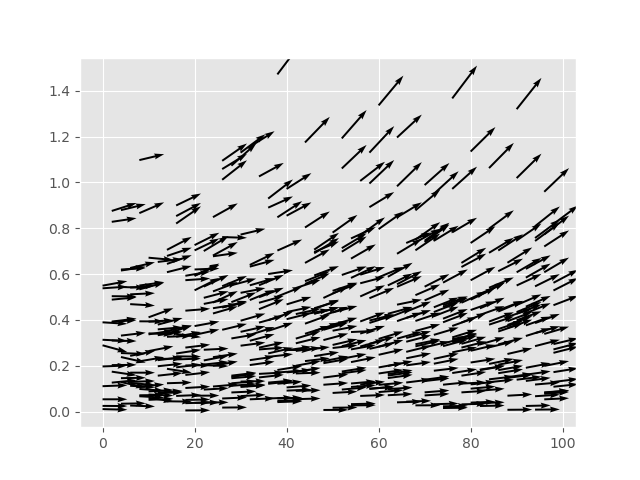
\includegraphics[width=0.45\linewidth]{figure/intensity_dynamic.png}\label{fig:muVector}}
%     \caption{Visualization of vector fields. a) is a vector field of the hidden state and b) is the vector field of $\mu(t;e_i)$. The length of the arrow represents the magnitude.}
%     \label{fig:vectorfields}
% \end{figure}
% % \vspace*{3in}

% \subsection{Visualization of Continuous Dynamics}
\begin{figure}[!h]
    \centering
    \subfigure[Visualization of $\mu(t;e_i)$ trained using MOOC.]
    {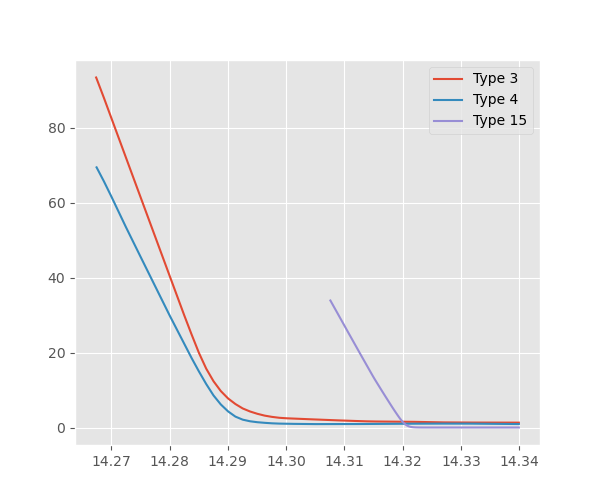
\includegraphics[height = 0.4\textwidth]{figure/mooc_inten.png}}
    \hfill
    \subfigure[\raggedright $\hat{f}(t;e_{i})$ trained using in MOOC.]
    {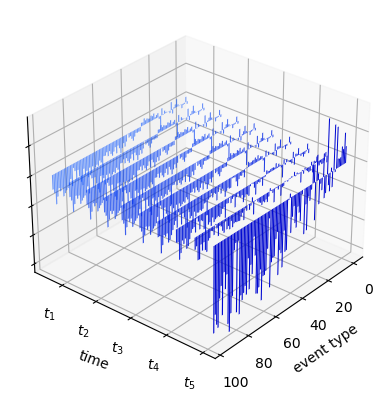
\includegraphics[height = 0.4\textwidth]
    {figure/mook_fk_14.png}}

    % \vspace{-0.3cm}
    \subfigure[$\mu(t;e_i)$ trained using Reddit.]
    {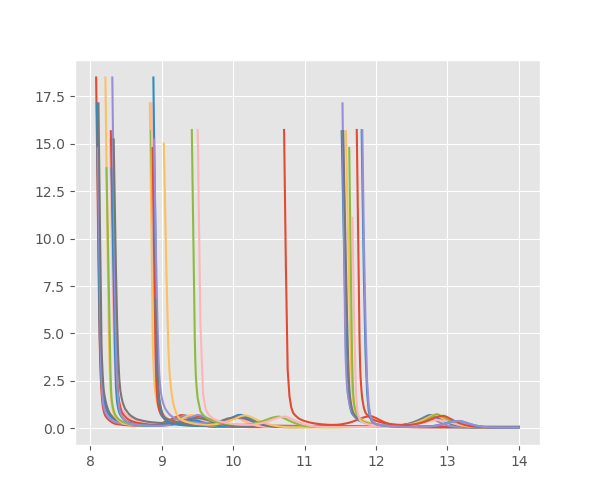
\includegraphics[height = 0.4\textwidth]{figure/reddit_inten.png}}
    \hfill
    \subfigure[\raggedright $\hat{f}(t;e_{i})$ trained on Reddit dataset.]
    {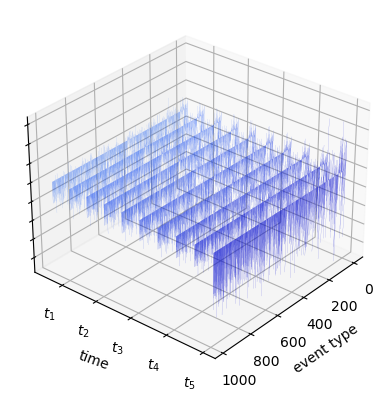
\includegraphics[height = 0.4\textwidth]
    {figure/reddit_fk_148.png}}
    \caption{Visualization of dynamics of $\mu$ and $\hat{f}$ in benchmark dataset. (a) is a visualization of ground intensity trained on MOOC dataset, (b) is a visualization of $\hat{f}(t;e_i)$ changing through time trained using MOOC dataset, (c) is a visualization of ground intensity trained on Reddit dataset, and (d) is a visualization of $\hat{f}(t;e_i)$ changing through time trained using Reddit dataset.}
\end{figure}

\begin{figure}[p] \ContinuedFloat
    \vspace{-10cm}
    % \vspace{-.3cm}
    \subfigure[Visualization of $\mu(t;e_i)$ trained using SO.]
    {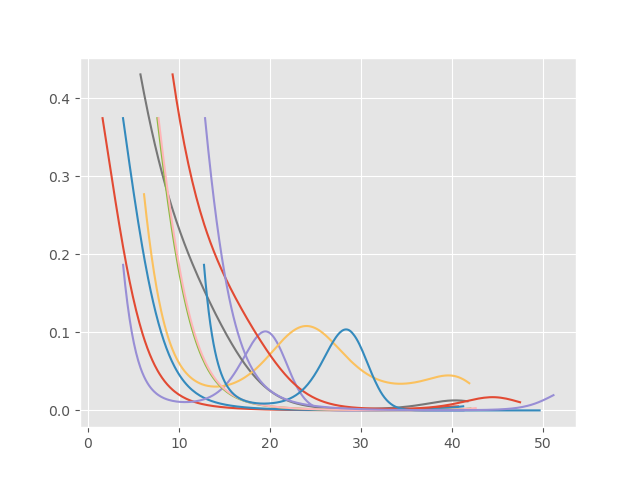
\includegraphics[height = 0.4\textwidth]{figure/SO_int.png}}
    \hfill
    \subfigure[\raggedright Visualization of $\hat{f}(t;e_{i})$ in MIMIC.]
    {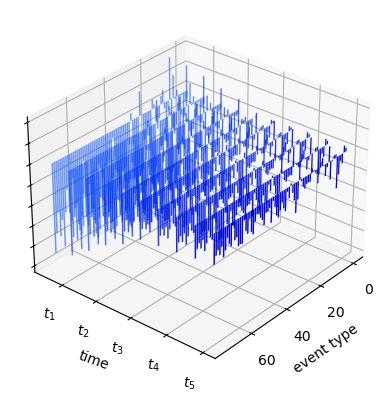
\includegraphics[height = 0.4\textwidth]{figure/mimic_fk_10.png}}
    \caption{Visualization of dynamics of $\mu$ and $\hat{f}$ in benchmark dataset. (a) shows dynamics of ground intensity trained using Stack Overflow dataset, and (b) shows $\hat{f}(t; e_i)$ changing through time trained using MIMIC-II dataset.}
    \label{fig:mooc}
\end{figure}
\clearpage



\chapter{Conclusion}
% In this work, we presented a novel framework for modeling MTPP, i.e., Dec-ODE,  
that decouples influence from each event for flexibility and computational efficiency. 
The Dec-ODE leverages neural ODE to model continuously changing behavior of influence from individual events, 
which govern the overall behavior of MTPP, and we proposed a training scheme 
for a linear Dec-ODE, which let the influences be efficiently computed in parallel. 
The proposed method was validated on five real-world benchmarks yielding 
comparable or superior results. 
Moreover, it provides explainability to the modeling,
which suggests significant potential for applications such as out-of-distribution detection and survival analysis. 
In this work, we introduced a novel framework for modeling MTPPs, referred to as Dec-ODE, which decouples the influence of each event to enhance flexibility and computational efficiency. The Dec-ODE utilizes neural ODEs to model the continuously evolving influence of individual events, which control the overall dynamics of the MTPP. Additionally, we proposed a training scheme for a linear Dec-ODE, enabling the efficient parallel computation of influences. The method was validated on five real-world benchmark datasets, demonstrating comparable or superior performance. Furthermore, it offers explainability in the modeling process, highlighting its potential for applications in areas such as out-of-distribution detection and survival analysis.


%%
%% 한글요약문 시작 (Korean summary)
%%
%% Note. 영문논문일 경우에만 필요하니 한글논문의 경우에는 작성하지 마십시오.
%%
\begin{summarykorean}
    사건의 종류와 발생 시간의 쌍으로 이루어진 데이터는 의료, 산업, 금융 등 다양한 분야에서 수집되고 사용되고있다.
이러한 시계열 데이터를 확률론적 과정으로 모델링을 한다면 정보를 분석하거나 미래에 발생할 정보들을 예측하는 것에 효과적으로 사용될 수 있다.
특히 사건의 발생 시간에 대한 예측을 위해 자주 사용되는 방법론으로는 Marked Temporal Point Process (MTPP) 가 있다.

이러한 MTPP를 인공지능을 활용하여 모델링하는 것에는 다양한 접근 방법이 제안되었다.
이중에서 대표적인 접근 방법들로는 RNN과 Transformer기반의 모델을 사용하는 방법들이 성능적인 측면에서 효과를 입증하였다.
특히 이러한 방법론들은 사건들 사이의 관계성을 학습하여 효과적인 예측을 하는 것을 장점으로하지만, 
모델이 어떠한 이유로 이러한 결과를 출력하였는지에 대한 설명성을 잃는 경우가 많다.
하지만 실제 생활에서는 다음 사건의 예측 뿐 아니라, 영향력에 대한 분석, 생존분석, 그리고 사건의 확률 분포에 대한 이해 등 다양한 활용이 요구된다.
다양한 분야에 활용되기 사건의 개별적인 영향력을 파악하는 것은 큰 중요성을 갖는다.

이러한 문제점을 해결하고자 본 논문은 이벤트들의 개별적인 영향력을 표현하는 프레임워크를 제안하였다.
각 영향력은 상미분방정식을 통해 모델링되고, MTPP에 대한 특성을 미분방정식의 특성을 활용하여 효율적으로 계산을 하는 방법론 또한 함께 제안하였다.
마지막으로 제안된 프레임워크의 효과성을 입증하기 위하여 단순한 구조를 갖는 모델과, 해당 모델을 활용한 더 효율적인 학습 방법을 제안하였다.

이벤트의 영향력을 설명가능하게 표현하기 위해 각각의 이벤트는 독립적인 시간에 따라 변화하는 프로세스로 표현된다.
이때 보다 효율적인 계산을 위해 다차원 프로세스를 상미분방적식으로 표현한다.
이 프로세스는 이벤트의 발생 시간에 대한 확률 분포를 계산하기 위한 $\mu$와 이벤트의 종류의 분포를 계산하기 위한 $\hat{f}$로 변환되게 된다.
시간에 대한 효율적인 예측을 위해 확률분포, 생존률 등의 예측값들의 시간에 따른 적분 값들은 미분방정식을 활용하여 프로세스와 함께 계산한다.
이렇게 독립적으로 모델링을 하는 것은 예측을 하는 것에 원하는 이벤트의 집합을 고려할 수 있는 장점을 제공한다.

이러한 방법론의 효과성을 보이기 위해 과거의 영향을 선형 합산 등 단순한 함수를 통해 관심 시점의 값을 계산하는 구현을 제안하였다.
이렇게 단순한 구현하는 것의 장점으로는 학습시 적분을 위해 모든 시작 시점부터 순차적으로 계산을 하는 것이 아니라, 
각각의 이벤트를 자신의 시점에 맞추어 동시에 계산 후 추후 손실함수 계산을 위해 사용 될 수 있다.

해당 프레임워크는 설명가능하고 연속적인 MTPP의 모델링을 하는 것 뿐 아니라, 
최고 성능을 내는 기존 방법론보다 좋거나 유사한 성능을 보이는 것을 보였다.
또한 제안된 방법론의 효율성 및, 프레임워크의 확장성이 실험을 통해 확인 되었다.

\
\end{summarykorean}

%%
%% 참고문헌 시작
%% Refences
%%

\bibliographystyle{unsrt}
\bibliography{mybib}

%%
%% 감사의 글 시작
%% Acknowledgement
%%
% @command acknowledgement 감사의글
% @options [default: 클래스 옵션 korean|english ]
% - korean : 한글타이틀 | english : 영문타이틀

\acknowledgement[korean]
% 느낀점 배운점
새로운 도전을 할 수 있게 장려해주신 김원화 교수님 감사합니다. 교수님의 지도를 통해 항상 새로운 경험을하고 성장하기 위해 포기하지 않고 도전 할 수 있었습니다.
교수님의 지도를 통해 연구가 무엇인지에 대한 깊은 고찰을 할 수 있었습니다. 교수님께서 주신 가르침을 잊지 않겠습니다.

또한 연구실 동료들에게도 함께하며 많은 도움을 받았기에 감사드립니다.
현아 - 연구자로서 본분을 다하는 모습을 보고, 저 또한 나태해지지 않고 많이 배울 수 있었습니다.
지은 - 바라는 바를 뚜렷하게 표현하고, 긍정적으로 노력하는 모습.
승훈 - 맡은바에 최선을 다하는 모습. 힘든 상황에서도 긍정적인 태도로 대하는 모습.
준혁 - 묵묵히 정진하는 모습. 스스로를 고찰하며 발전해 나아가는 모습.
유빈 - 누구보다 섬세하고 주변 사람 모두 고려하는 모습.
재윤 - 못하는 것 없고, 쉬지 않고 발전해 나아가는 모습.
수연 - 감정에 치우치지 않고, 멋진 연구를 하는 모습.
예찬 - 넓은 시야를 갖고, 주변사람들을 배려하고 배우는 자세.
민재 - 새로운 시각을 제시하고, 주변을 즐겁게 해주는 모습. 연구를 할때에 연구를 이해하고자 하는 모습.
성우 - 이론적인 베이스를 위해 끊임 없이 공부하고 학습하는 모습에 정말 큰 자극을 많이 받았습니다. 제가 추구하는 연구의 방향성에도 항상 영향을 받았습니다.
세형 - 연구를 대하는 자세에대해 많이 배웠습니다. 정말 멋있는 연구 많이 하기를 기대합니다.
동현 - 함께 연구를 하며 다재다능한 능력에 큰 도움이 되었습니다. 저의 연구에 도움을 준 것 만큼 제가 연구하는 것에 큰 도움이 되었으면 합니다.
성윤 - 정말 현명하고, 한편으로는 선배같은 동료였습니다. 
민재 - 긍정적인 태도와 밝은 모습으로 연구실 생활에 큰 도움을 받았습니다.
하영 - 씩씩하게 새로운 것을 배우고자 하는 태도, 긍정적인 에너지를 통해 힘들때 큰 도움이 되었습니다.
수진 - 성실하고 쾌활하게 연구하는 모습을 통해 즐겁게 연구할 수 있었습니다.
승주 - 새로운 주제를 공부하고, 함께 의견을 나누며 흥미로운 주제를 고민하고 알아갈 수 있었습니다.
재진 - 한학기 밖에 함께하지 못해 정말 아쉽습니다.
%%때로는 엄하고 때로는 부드러운 모습으로 지도 해주신 한준희 교수님, 감사드립니다.
%%
%% 이력서 시작
%% Curriculum Vitae
%%
% @command curriculumvitae 이력서
% @options [default: 클래스 옵션 korean|english ]
% - korean : 한글이력서 | english : 영문이력서
\curriculumvitae[english]

    % @environment personaldata 개인정보
    % @command     name         이름
        % input data only you want
    \begin{personaldata}
        \name       {Yujee Song}
    \end{personaldata}

    % @environment education 학력
    % @options [default: (none)] - 수학기간을 입력
    \begin{education}
	\item[2023. 02.\ --\ 2025. 02.] Graduate School of Artificial Intelligence, POSTECH (M.S.)
	\item[2020. 03.\ --\ 2022. 02.] Computer Science \& Engineering, Chung-Ang University (B.S.)
	\item[2015. 09.\ --\ 2017. 06.] Computer Science \& Engineering, UC Irvine (B.S.)
    \end{education}

    % @environment experience 경력
    % @options [default: (none)] - 해당기간을 입력
   \begin{experience}
	\item[2024. 07.\ --\ 2024. 09.] Medical AI Research \& Development Intern, VUNO
	\item[2023. 02.\ --\ 2025. 02.] Medical Information Processing Lab, Graduate School of Artificial Intelligence, POSTECH
   \end{experience}

    % @environment activity 학회활동
    % @options [default: (none)] - 활동내용을 입력
%    \begin{affiliation}

%    \end{affiliation}

    \afterpage{\blankpage}  % 마지막장 백색별지

%% 본문 끝
\end{document}
